% !TeX root = ../main.tex

\subsection{开发方法}

\begin{enumerate}
	\item{面向对象开发}
	\par 采用面向对象的开发方法,自底向上的归纳,将系统的各个部分抽象为不同的类。通过定义清晰的接口和实现详细的封装,
	降低模块之间的耦合度,提高系统的可扩展性和可维护性。

	\item{可视化开发}
	\par 采用可视化开发方法。由于三维重建和语义融合产生的模型数据抽象且数据量庞大,因此在开发过程中难以直接判断系统运行的正确性。
	因此,需要首先编写出可视化模块,以实时展示和检查点云生成及语义融合更新的过程。这不仅方便开发过程中识别和修复错误,还能直观地展示开发成果。

	\item{增量开发}
	\par 由于课题组对此系统的急切需求,因此采用增量开发的方法。首先依次实现室内重建、可视化、点云生成及语义融合更新等系统的核心功能。
	在核心功能稳定运行后,再逐步添加增量式重建、曲面重建和实例融合更新等额外功能。

	\item{编码规范}
	\par 遵循 \href{https://google.github.io/styleguide/cppguide.html}{Google C++ Style Guide} 编码规范以确保编写的代码能达到预期的功能并具有高可读性。
	每个头文件都需要使用宏定义来防止被多次包含,如 Matrix.h 需要声明为 MATRIX\_H\_,且每个头文件都是自足的,不依赖于其他头文件的包含顺序。
	命名规则方面,类名采用驼峰命名法,变量和函数名使用小写字母和下划线。
	初始化方面,应遵循RAII(Resource Acquisition Is Initialization)原则,尽量使用C++的标准类型。特别是对于如Space、Frame等负责管理资源的类,需要自定义构造函数和析构函数,同时禁用拷贝函数。
	为了线程安全,存在多线程竞争的地方,例如动画窗口、数据交换等,需要使用std::mutex进行同步。
\end{enumerate}

\subsection{实现效果}

\begin{figure}[htbp]
	\centering
	\subfigure[RGB图像]{
		\begin{minipage}[t]{0.48\linewidth}
			\centering
			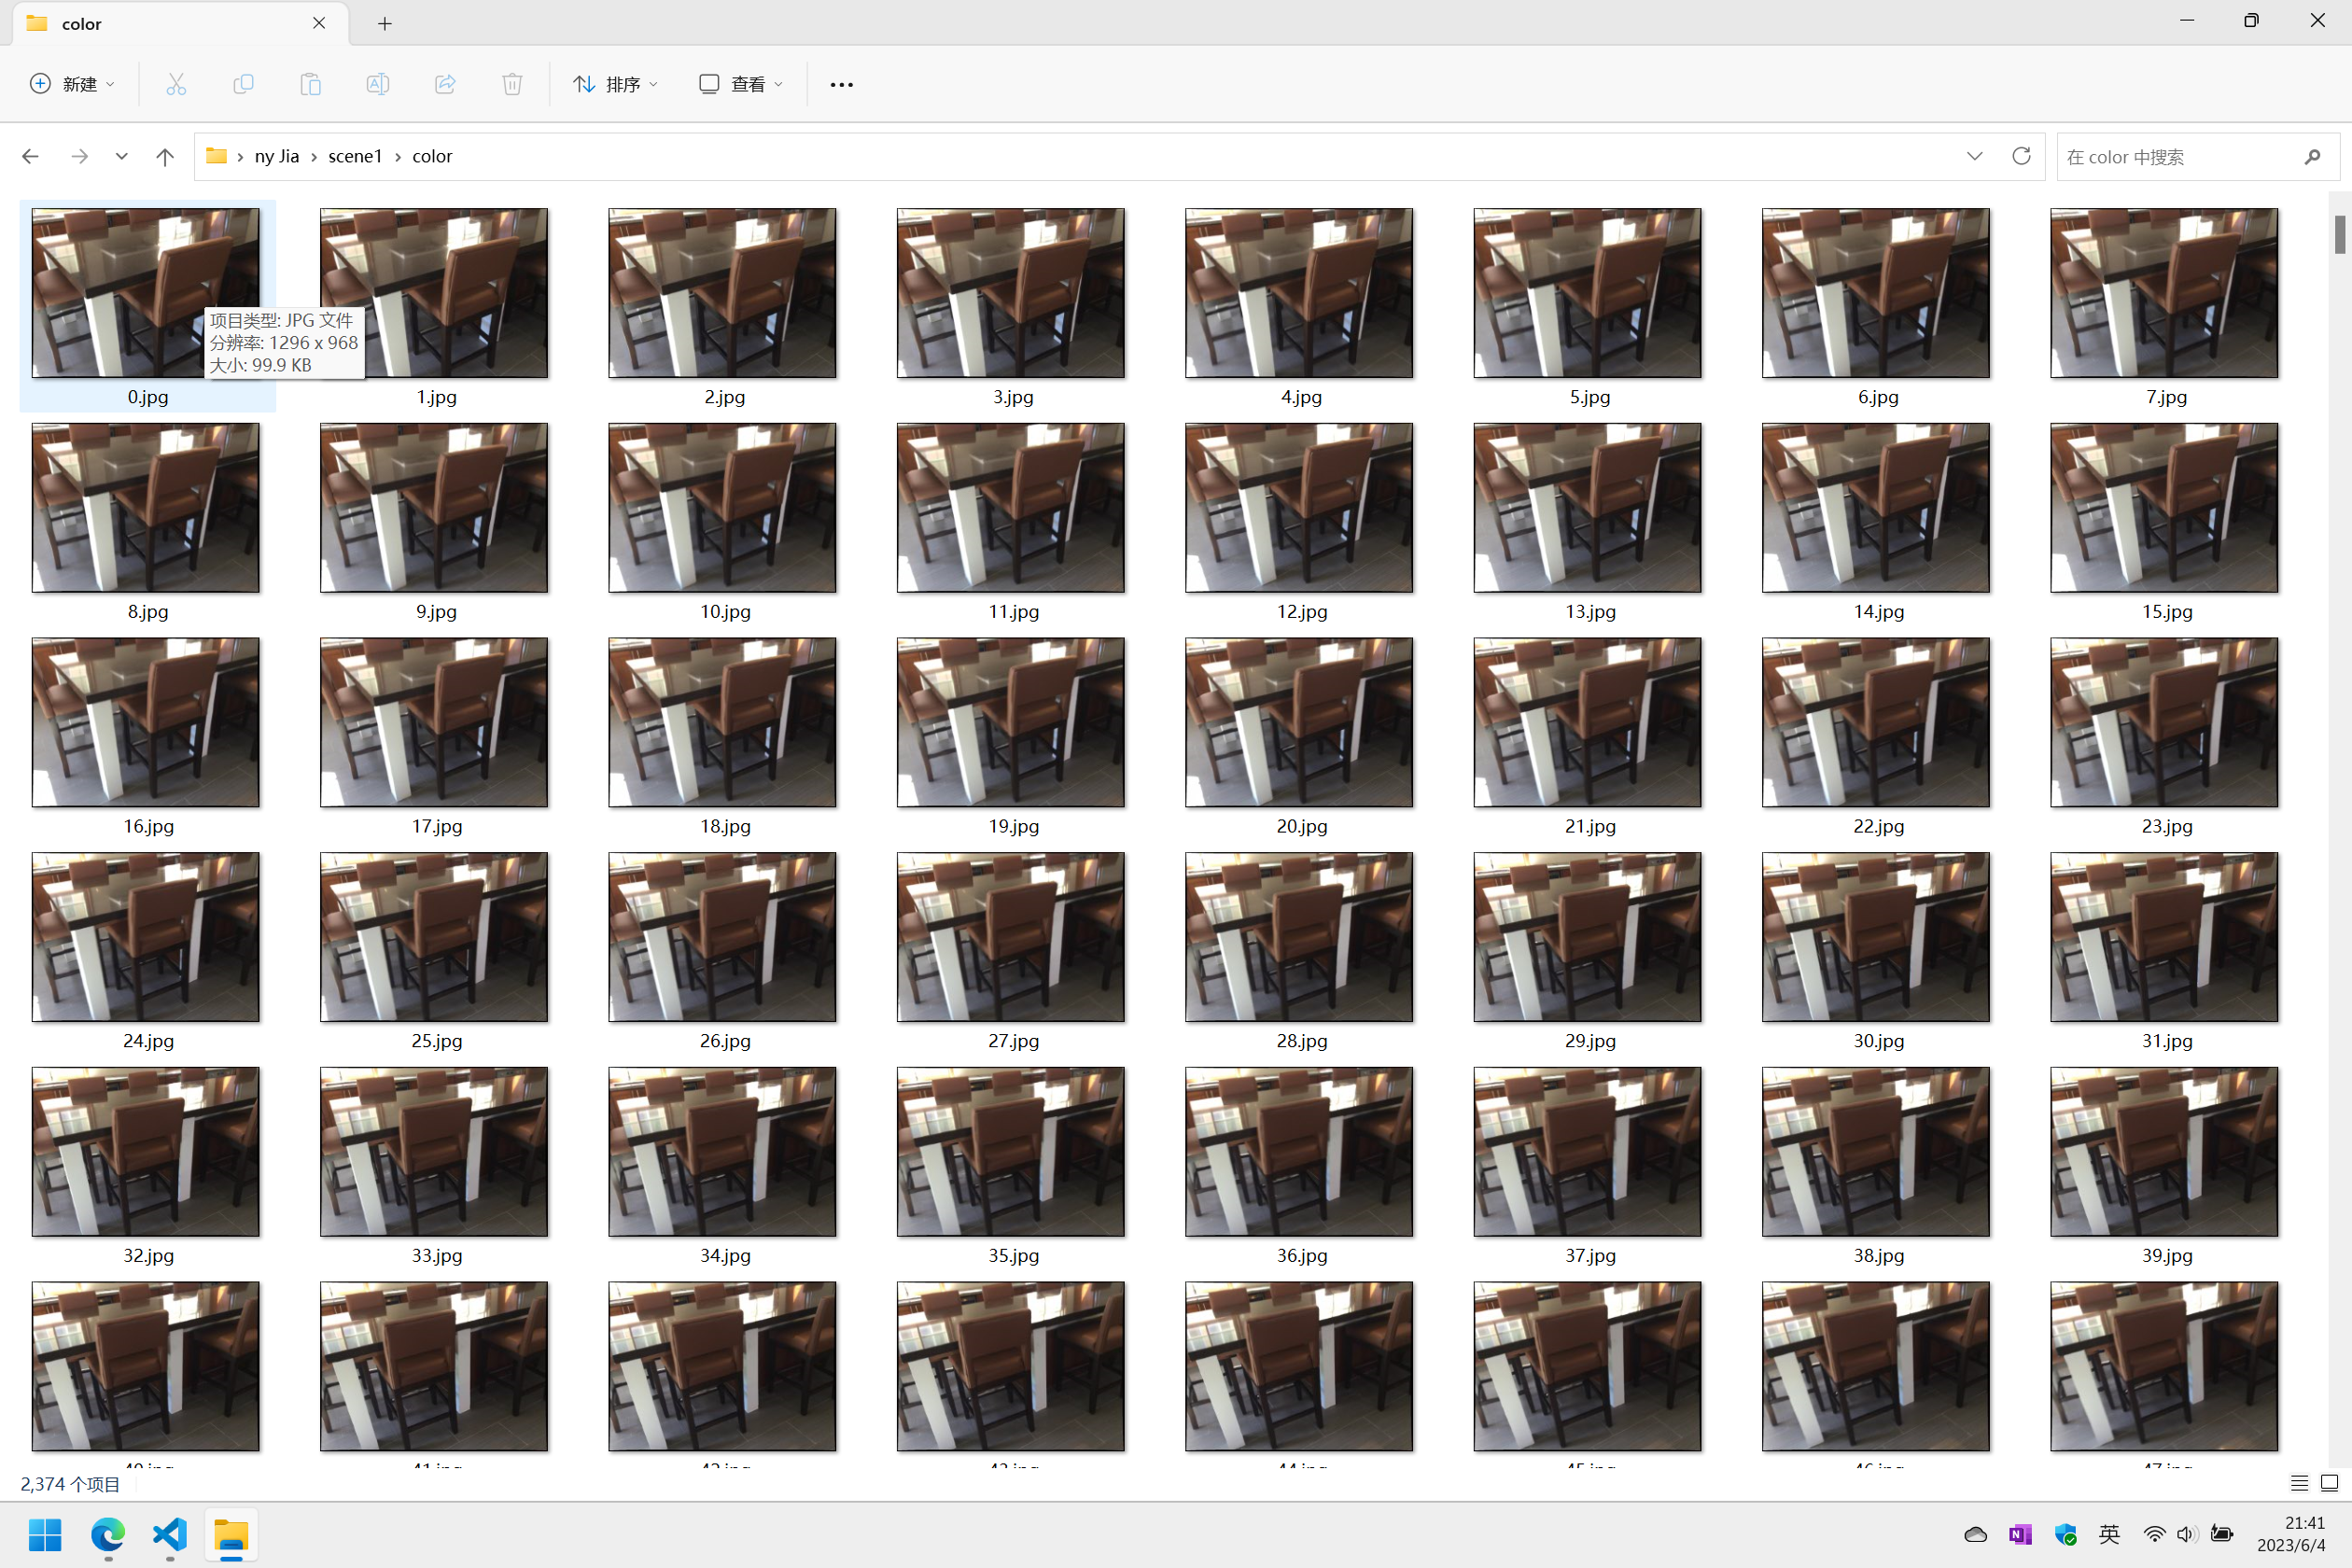
\includegraphics[width=1\textwidth]{figures/scene1_color.png}
		\end{minipage}
	}
	\subfigure[深度图像]{
		\begin{minipage}[t]{0.48\linewidth}
			\centering
			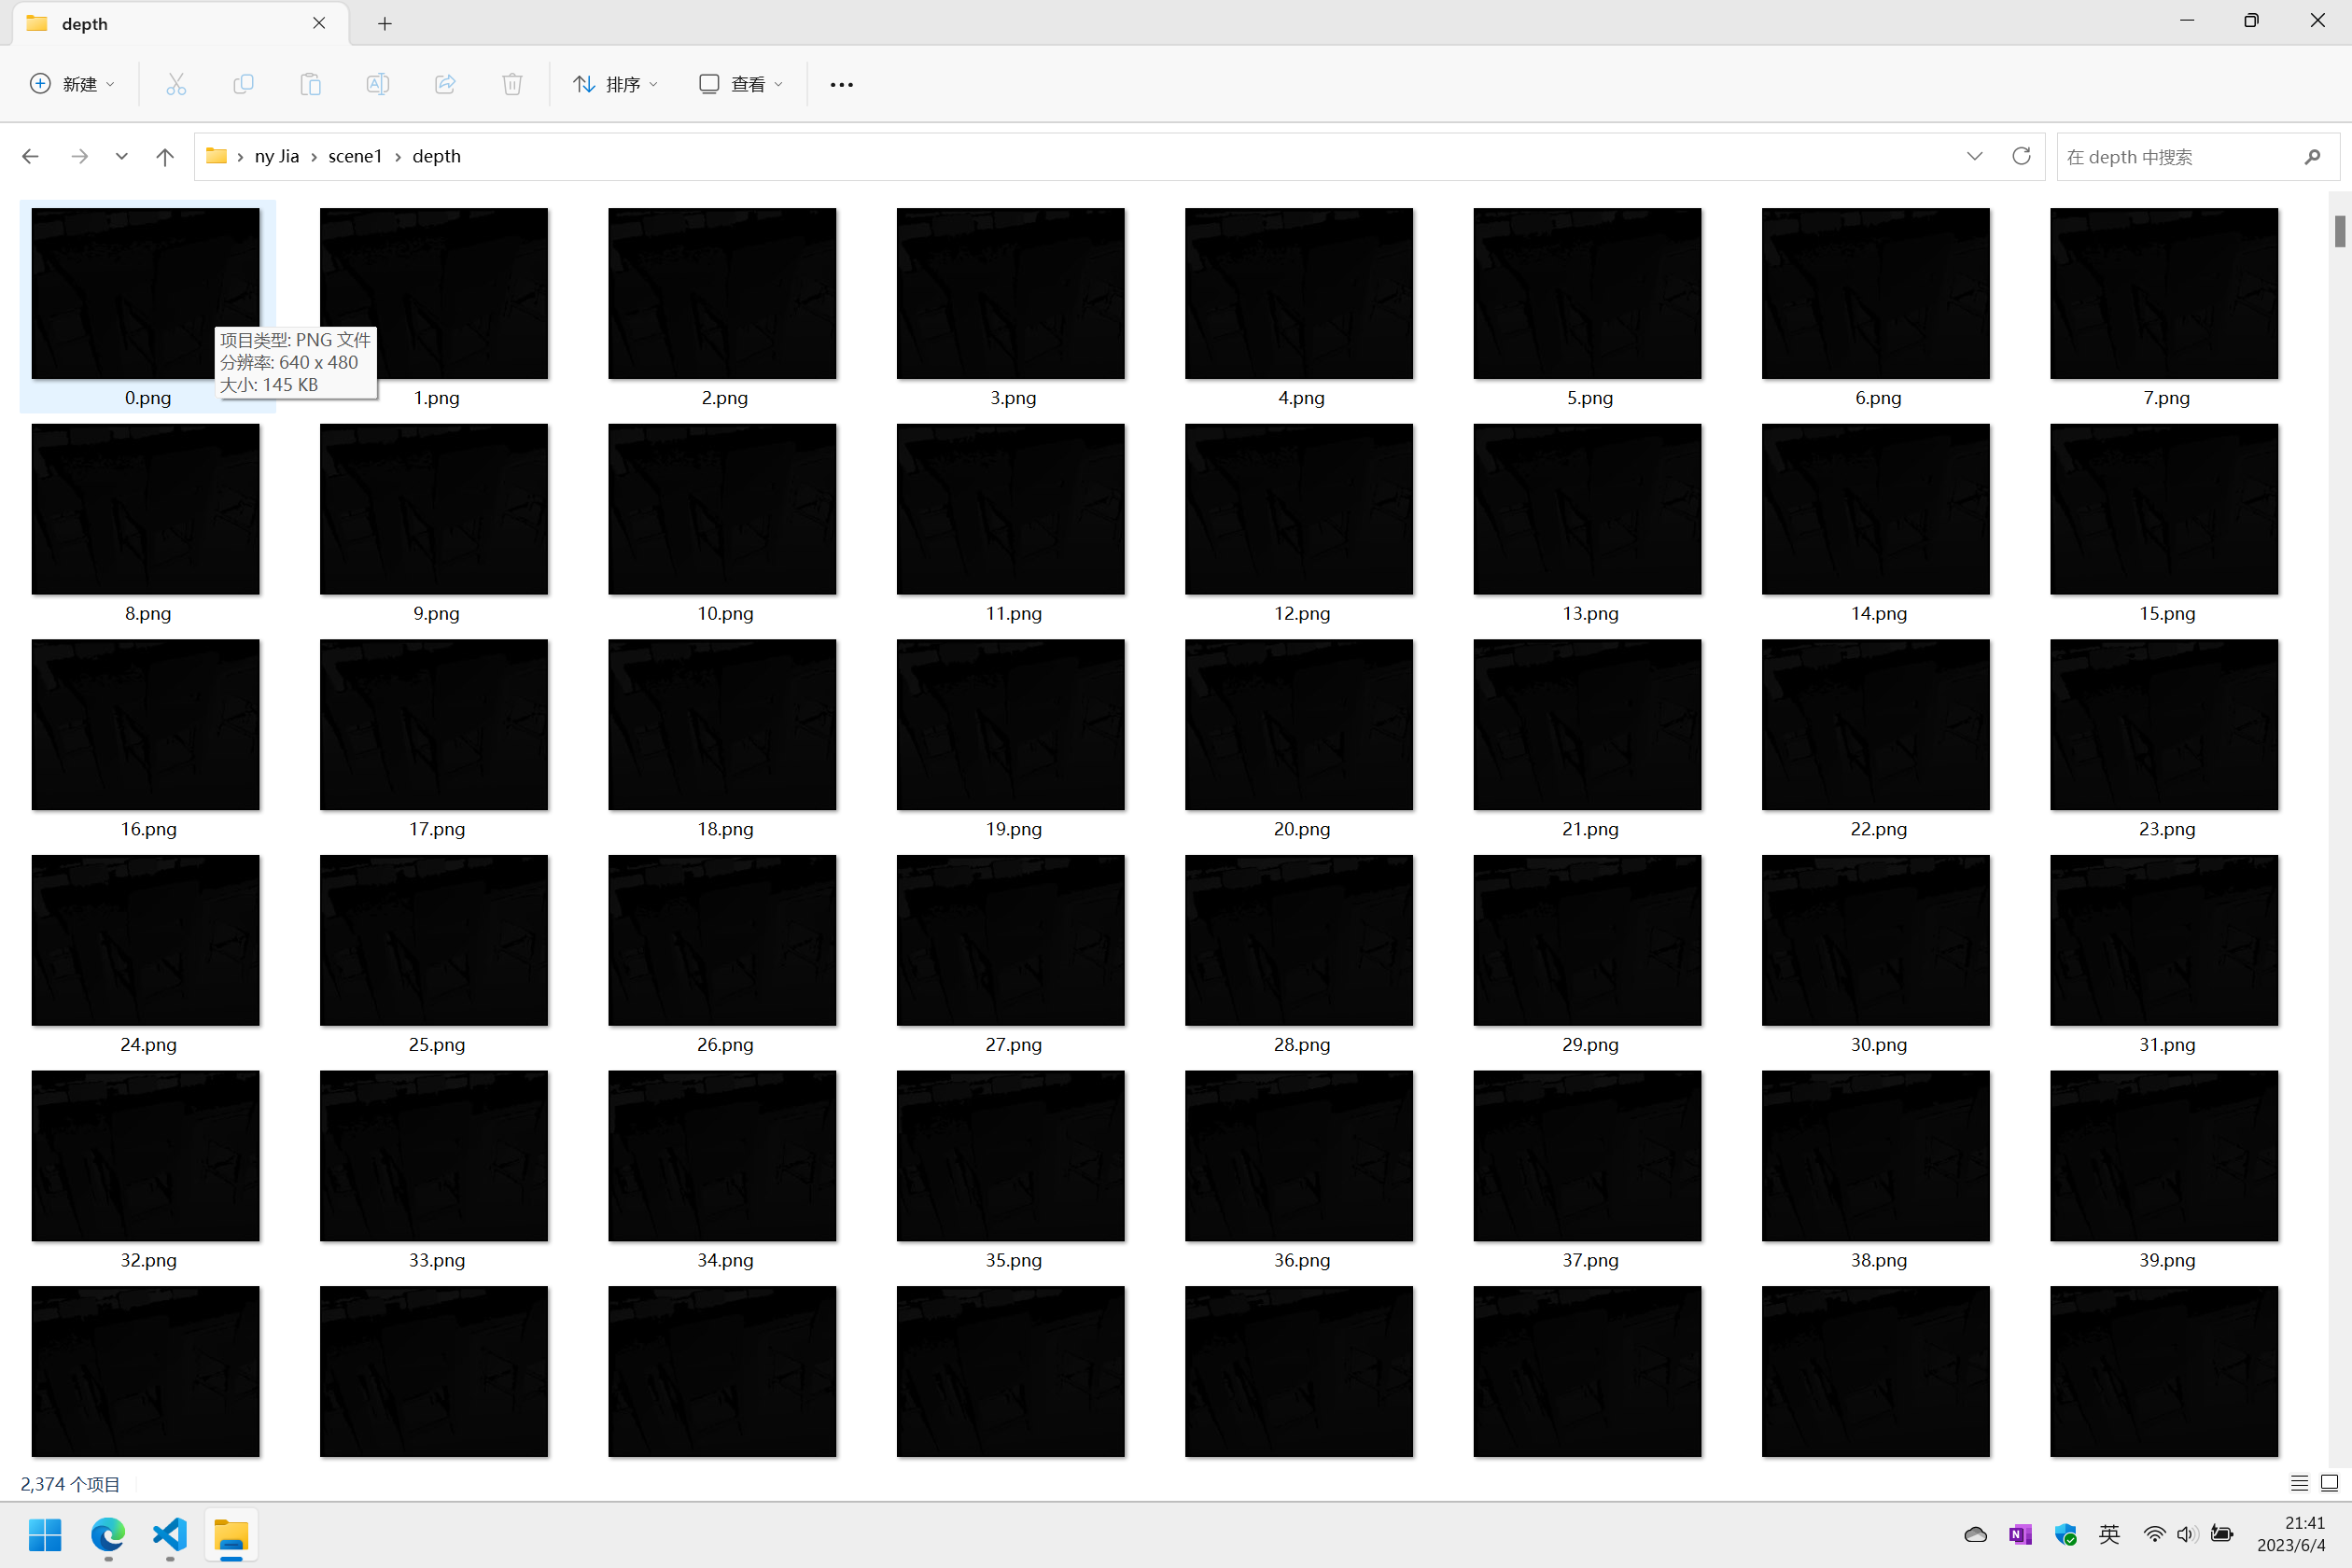
\includegraphics[width=1\textwidth]{figures/scene1_depth.png}
		\end{minipage}
	}
	\caption{数据采集结果}
	\label{fig:origin_img}
\end{figure}
\begin{figure}[htbp]
	\centering
	\begin{minipage}[t]{0.48\textwidth}
		\centering
		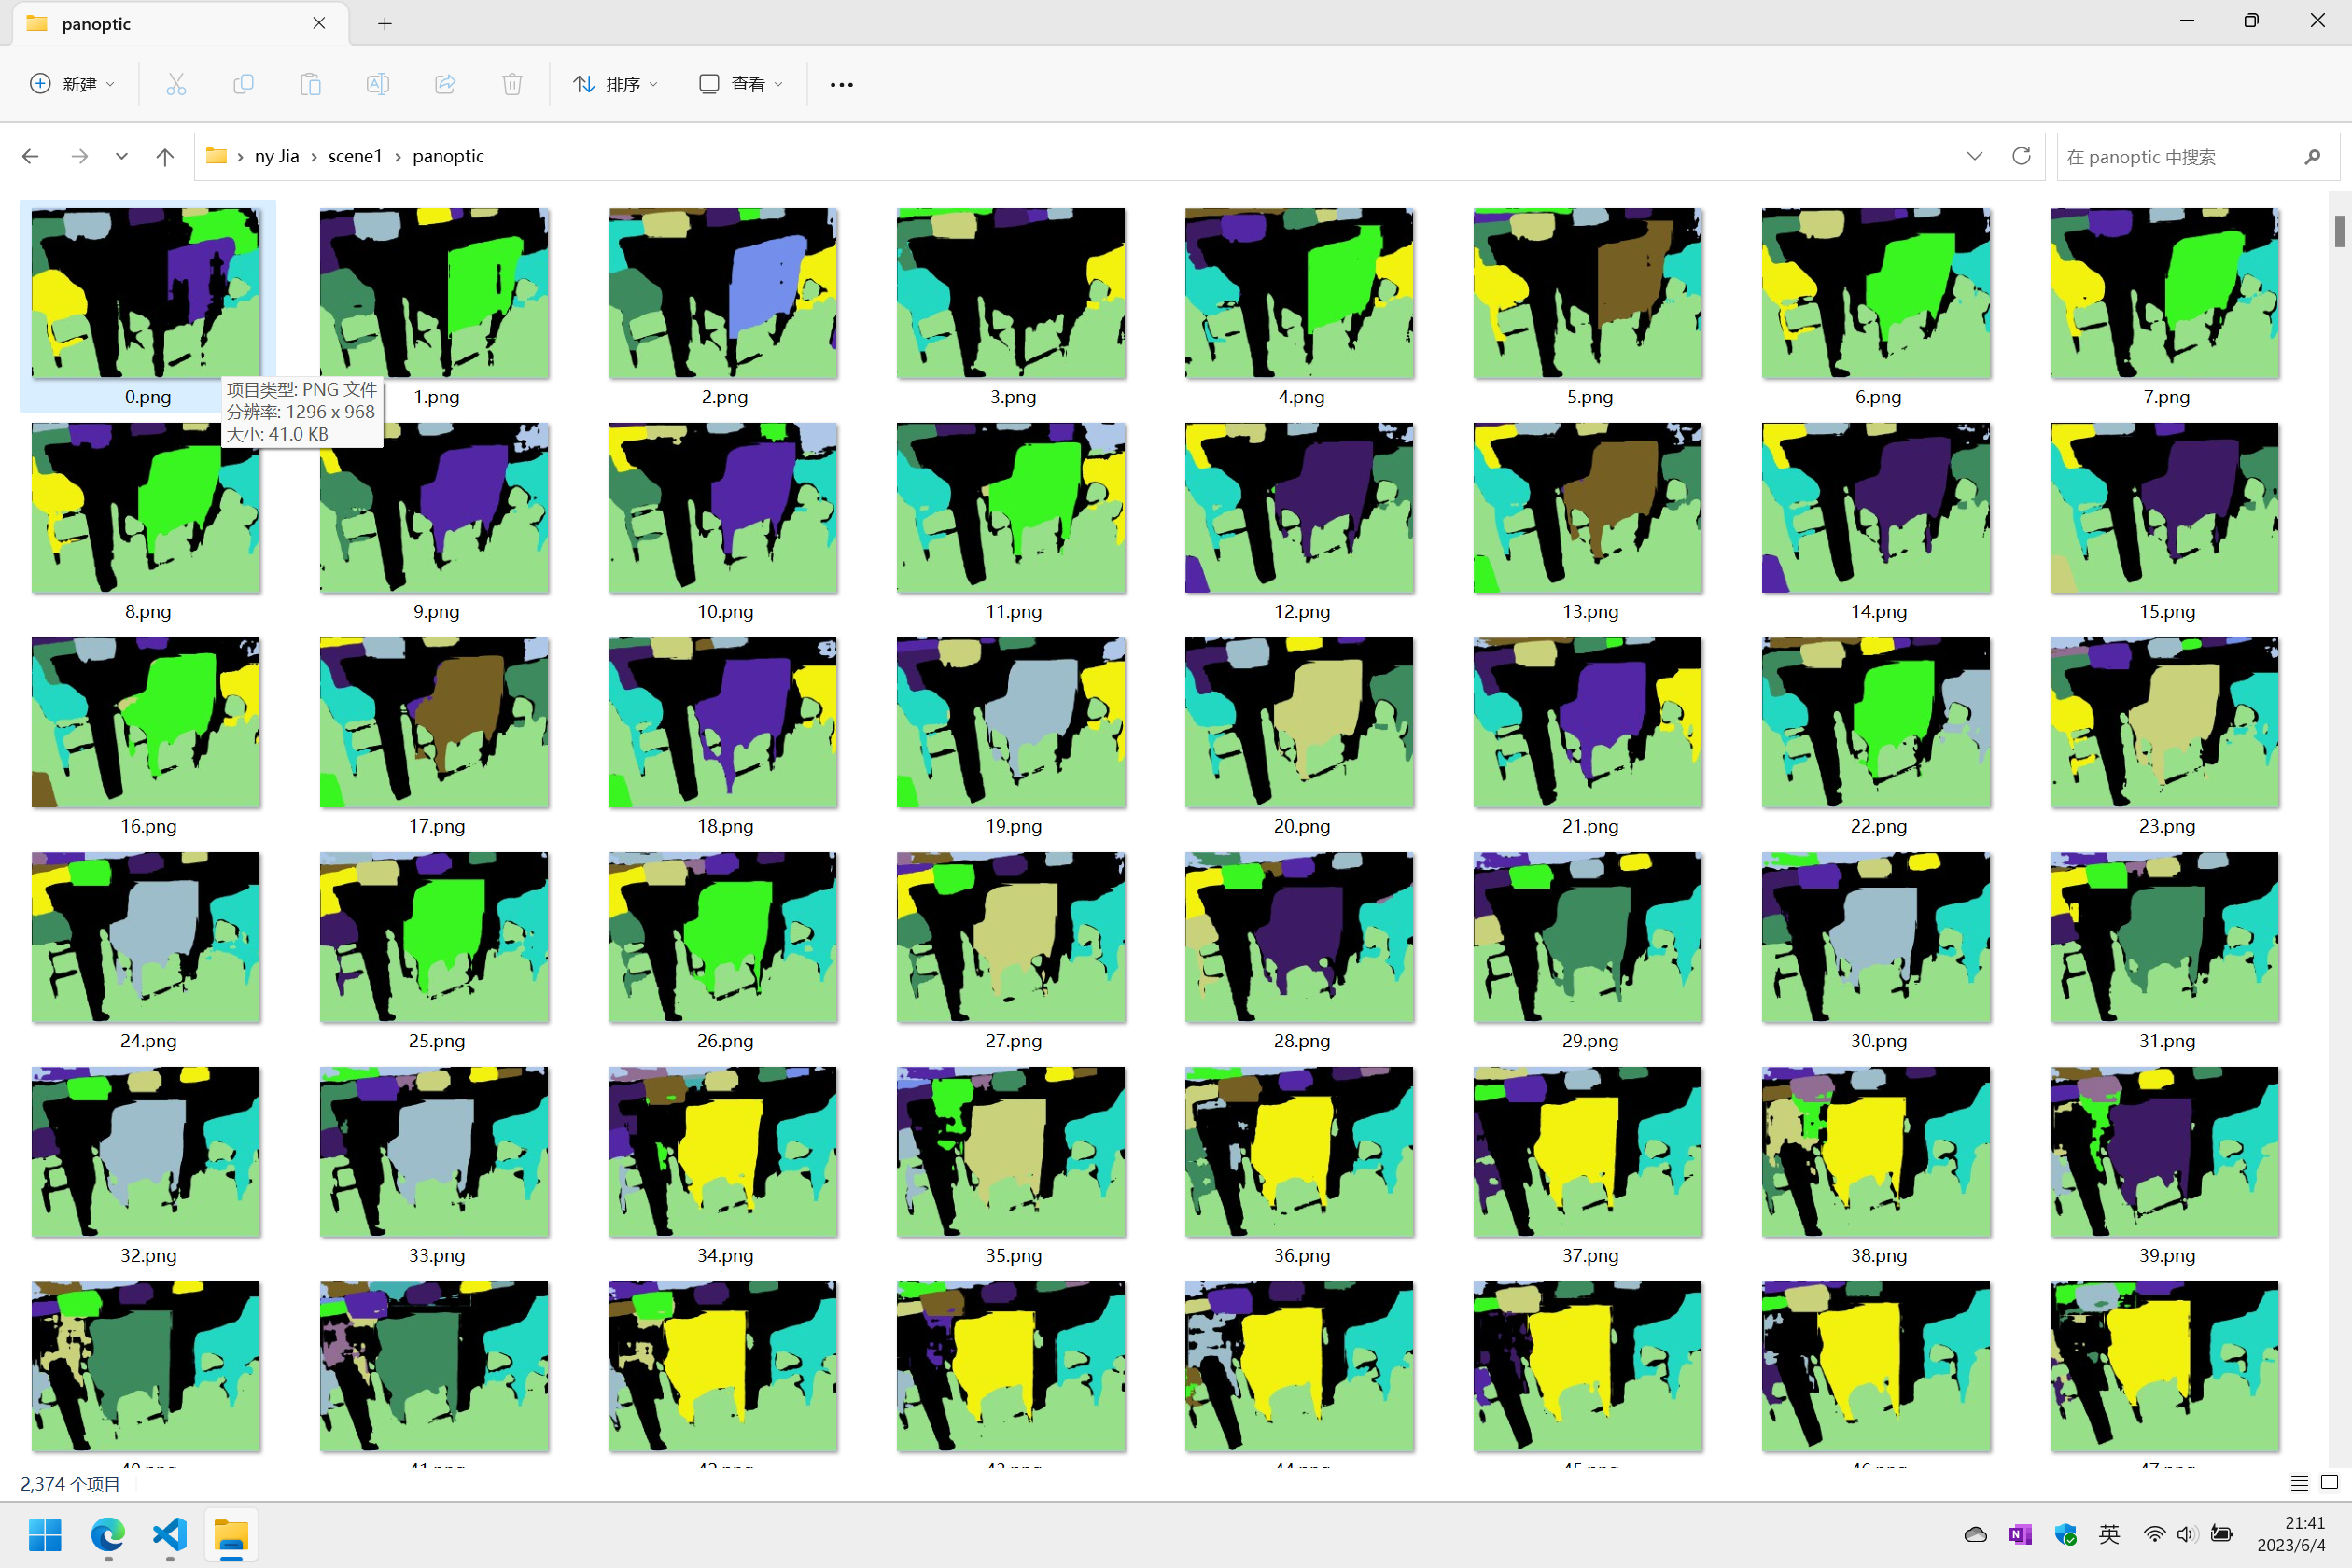
\includegraphics[width=1\textwidth]{figures/scene1_semantic.png}
		\caption{语义分割图像}
		\label{fig:seg_image}
	\end{minipage}
	\begin{minipage}[t]{0.48\textwidth}
		\centering
		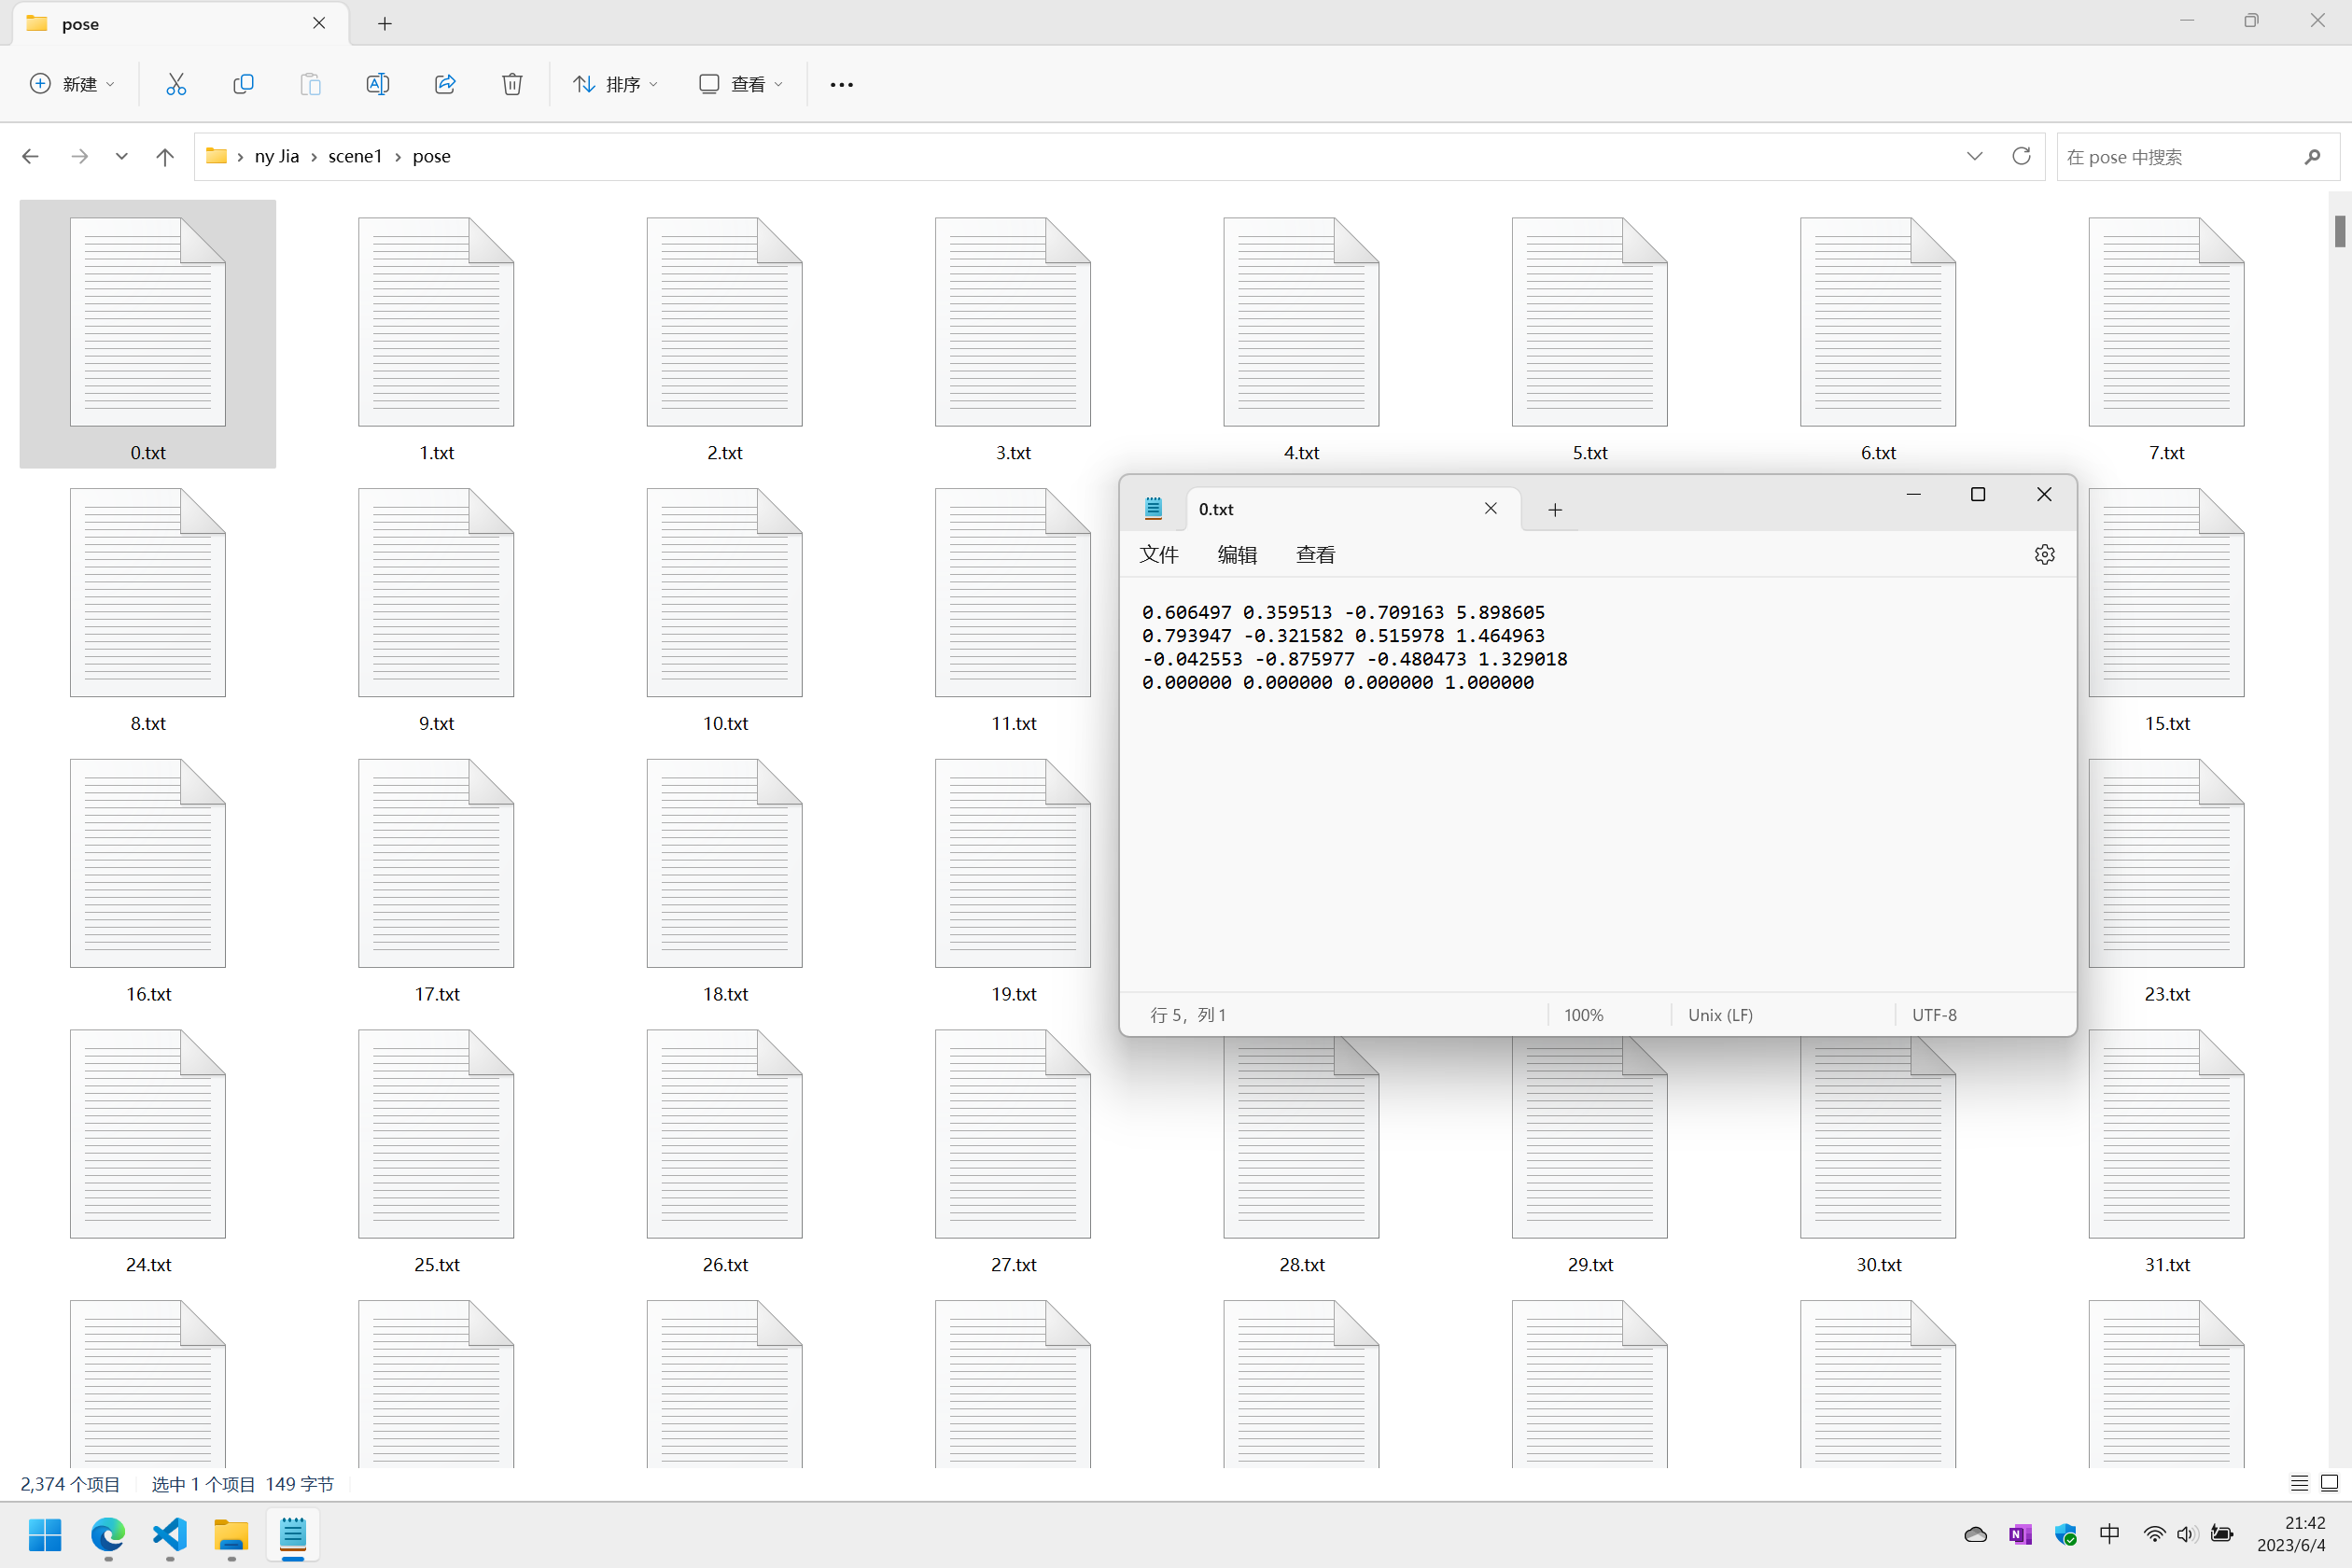
\includegraphics[width=1\textwidth]{figures/scene1_pose.png}
		\caption{位姿估计结果}
		\label{fig:pose_eval}
	\end{minipage}
\end{figure}

\par 图\ref{fig:origin_img}展示了 RGB-D 相机采集的视频流,每帧包括RGB图像和深度图像。其中,RGB图像可以看到环境的颜色和光照等。
\par 图\ref{fig:seg_image}展示了对RGB图像进行语义分割后的图像。每个像素都被赋予了一个语义标签,不同的标签通过不同的颜色表示出来。例如,黄色表示“椅子”,绿色表示“地板”等等。
\par 图\ref{fig:pose_eval}展示了对视频流的每帧图像进行相机位姿估计的结果。每个txt文件中有一个$4 \times 4$的矩阵,即当前帧对应的相机位姿矩阵。

\begin{figure}[htbp]
	\centering
	\subfigure{
		\begin{minipage}[t]{0.84\linewidth}
			\centering
			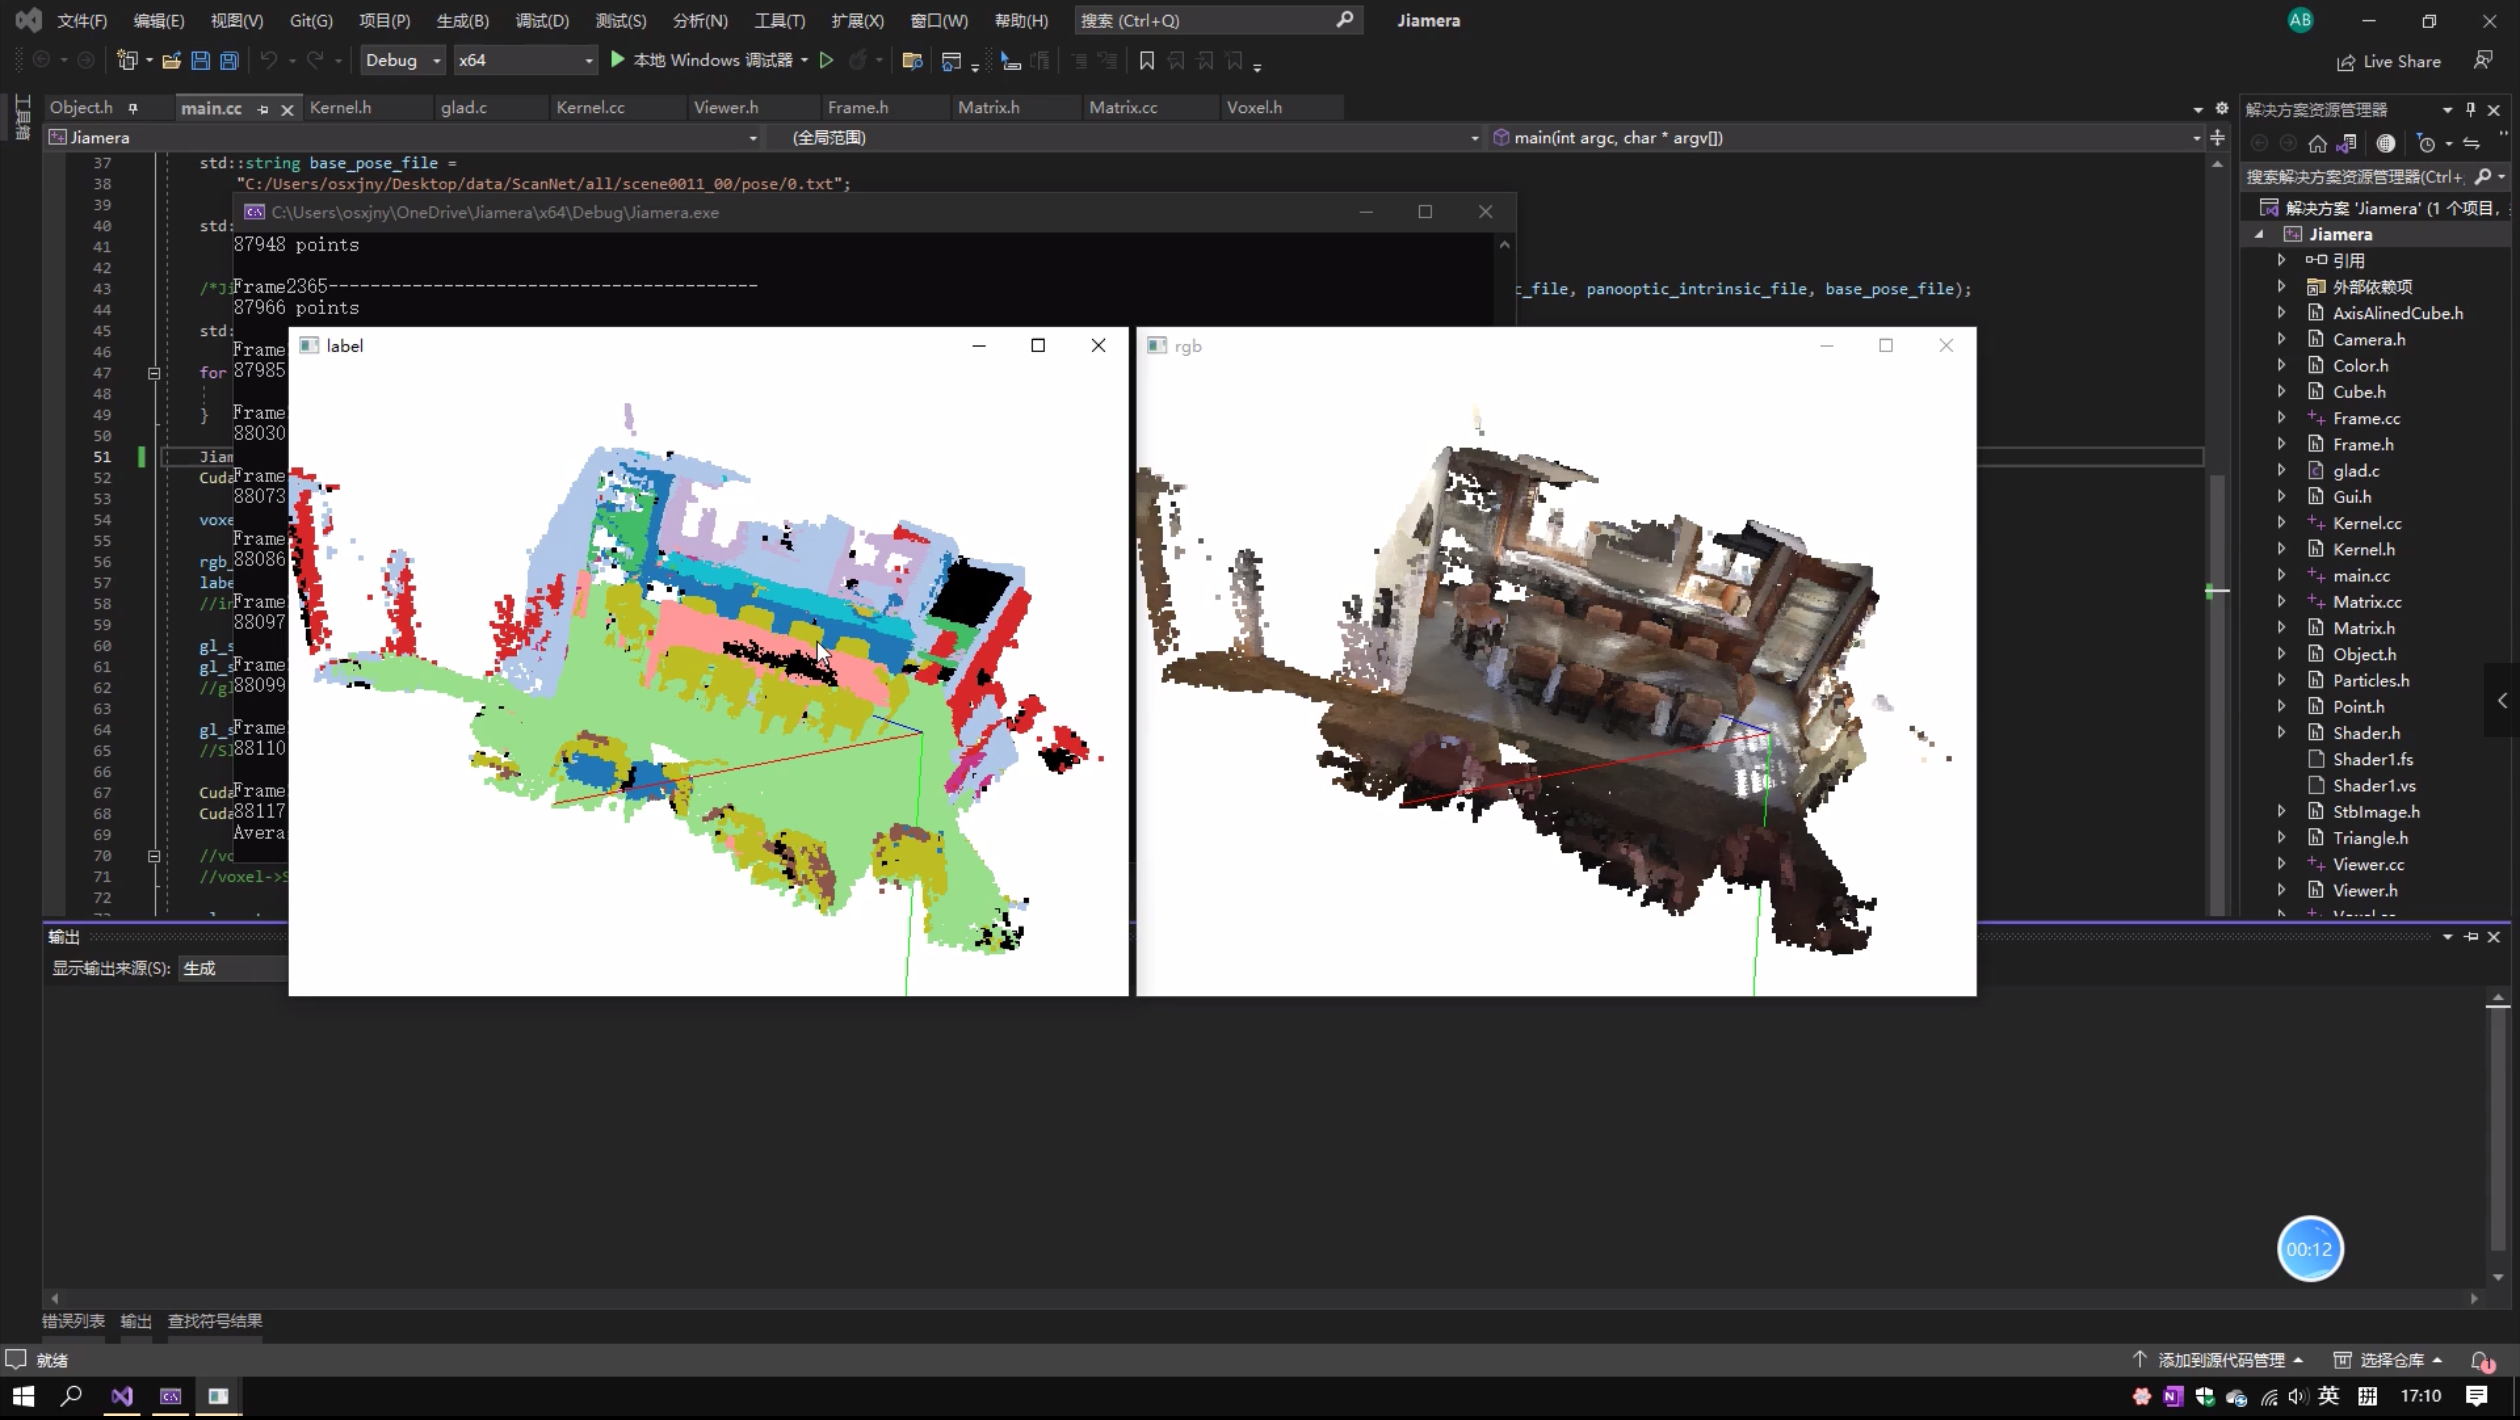
\includegraphics[width=1\textwidth]{figures/test_para/win_all_run.png}
		\end{minipage}
	}
	\caption{在Windows平台运行界面}
	\label{fig:run_result_windows}
\end{figure}

\par 图\ref{fig:run_result_windows}和图\ref{fig:run_result_ubuntu}展示了可视化模块的图形用户界面。这个界面可以清楚地看到物体的形状和位置,包含物体的RGB信息和语义信息。此外,用户可以通过键盘和鼠标输入对动画进行调整和控制,全方位实时观看三维重建的过程。

\begin{figure}[htbp]	
	\centering
	\subfigure[Ubuntu RGB动画]{
		\begin{minipage}[t]{0.48\linewidth}
			\centering
			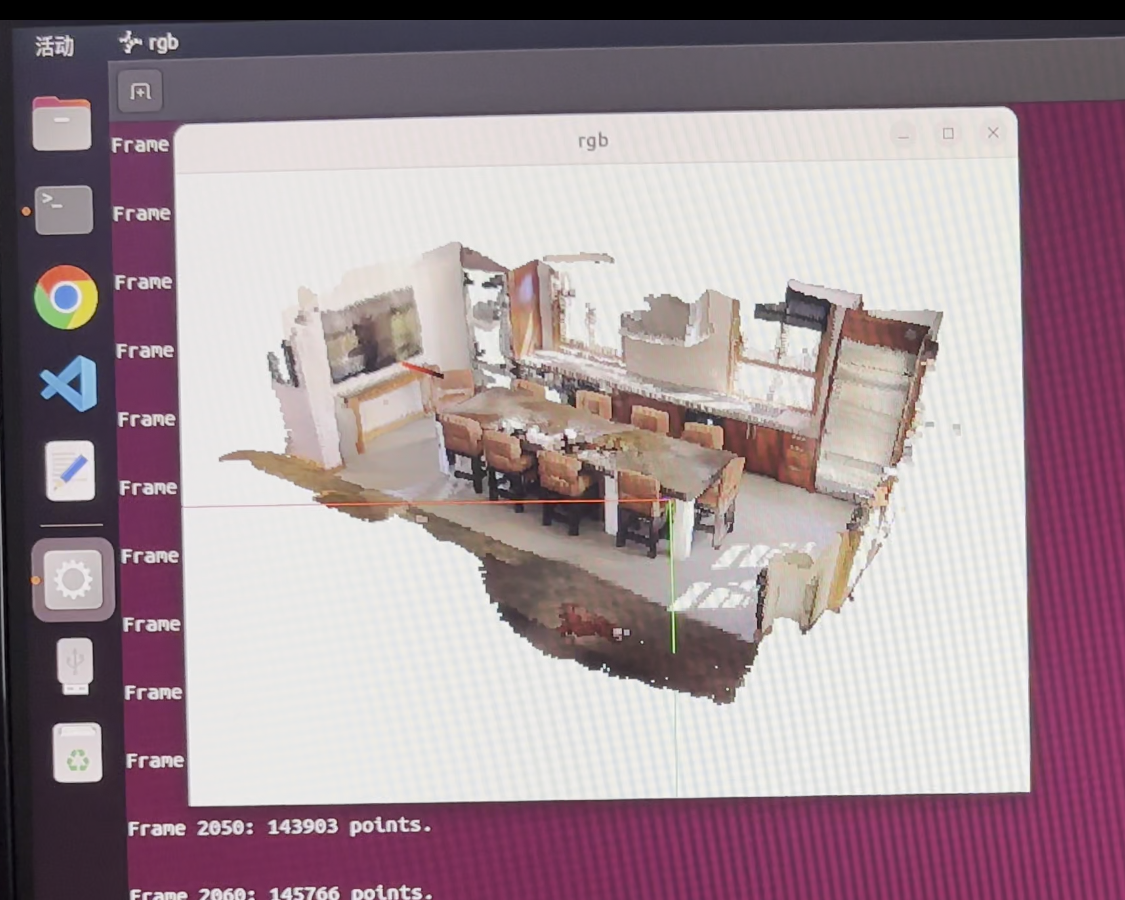
\includegraphics[width=1\textwidth]{figures/test_para/ubuntu_rgb_run.png}
		\end{minipage}
	}
	\subfigure[Ubuntu 语义动画]{
		\begin{minipage}[t]{0.48\linewidth}
			\centering
			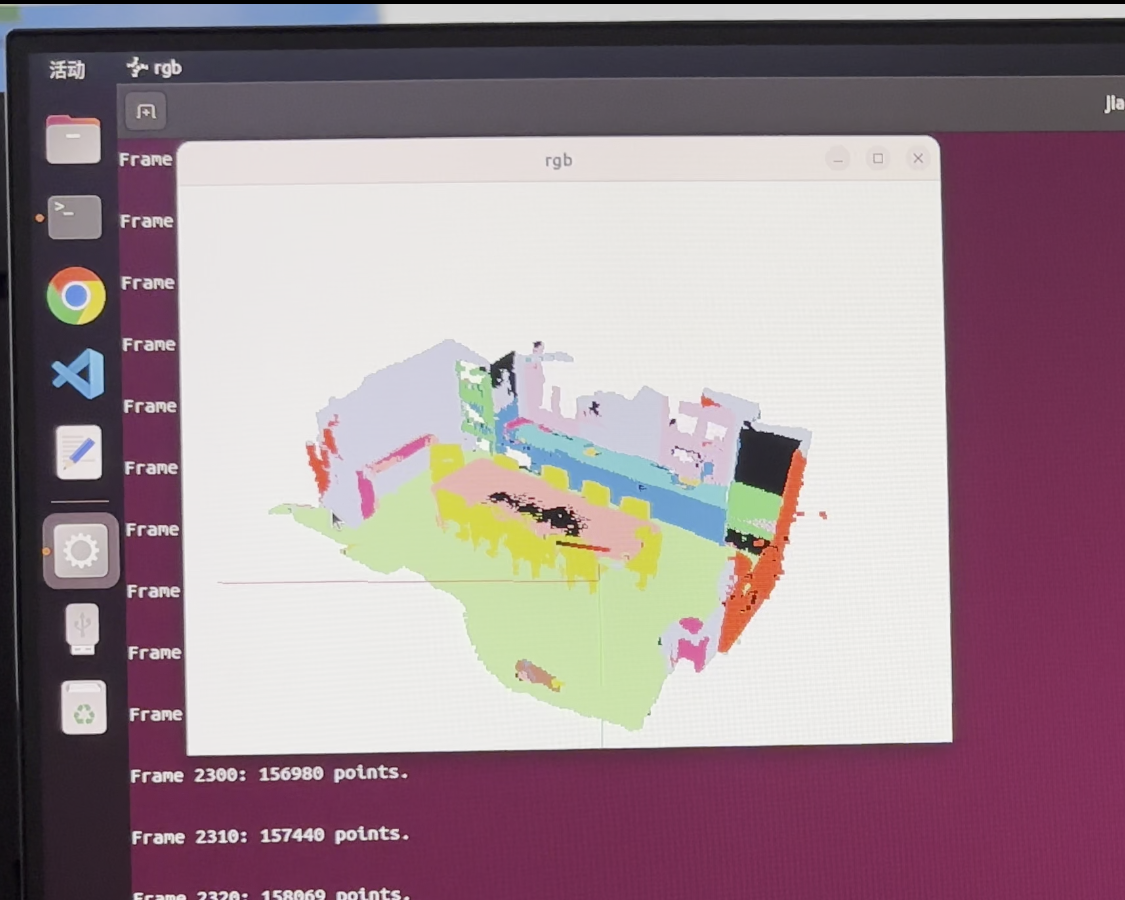
\includegraphics[width=1\textwidth]{figures/test_para/ubuntu_label_run.png}
		\end{minipage}
	}
	\caption{在Ubuntu平台运行界面}
	\label{fig:run_result_ubuntu}
\end{figure}

\par 图\ref{fig:export_result}展示了模型导出的结果。导出模型包括了每个点的三维坐标、RGB信息以及语义信息。

\begin{figure}[htbp]
	\centering
	\subfigure[RGB信息2cm模型]{
		\begin{minipage}[t]{0.48\linewidth}
			\centering
			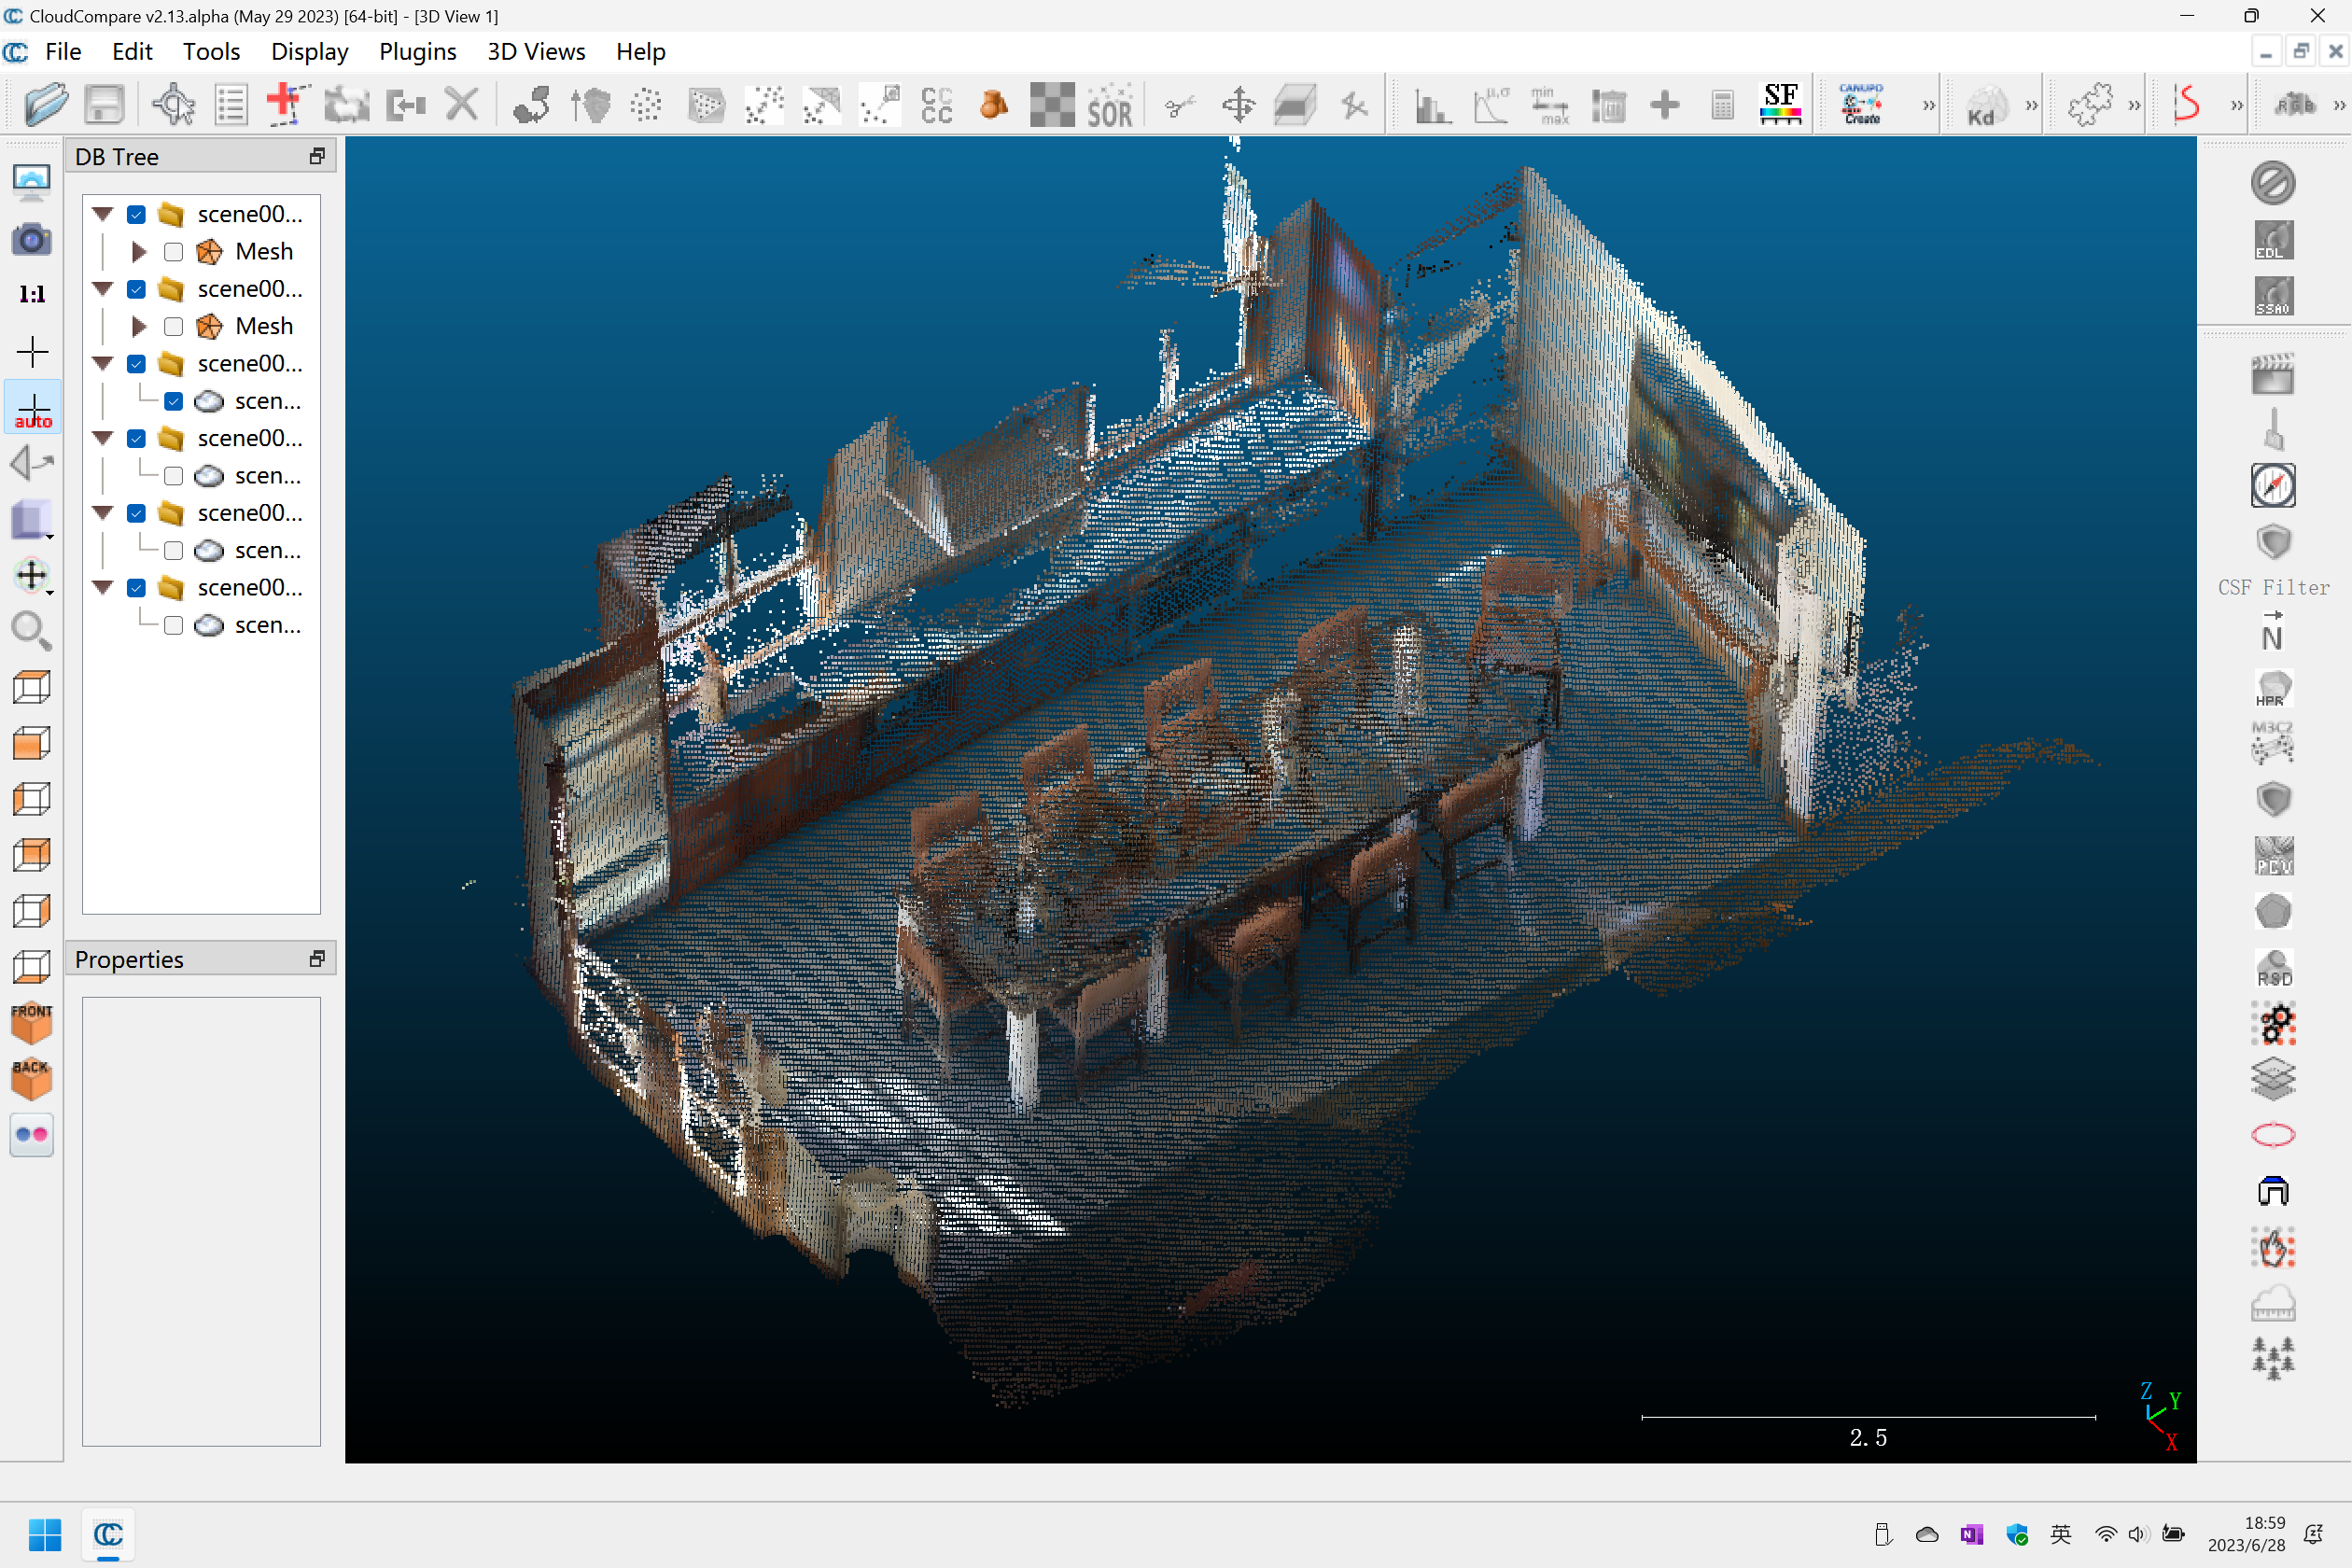
\includegraphics[width=1\textwidth]{figures/result/scene0011_rgb_2cm.png}
		\end{minipage}
	}
	\subfigure[RGB信息5cm模型]{
		\begin{minipage}[t]{0.48\linewidth}
			\centering
			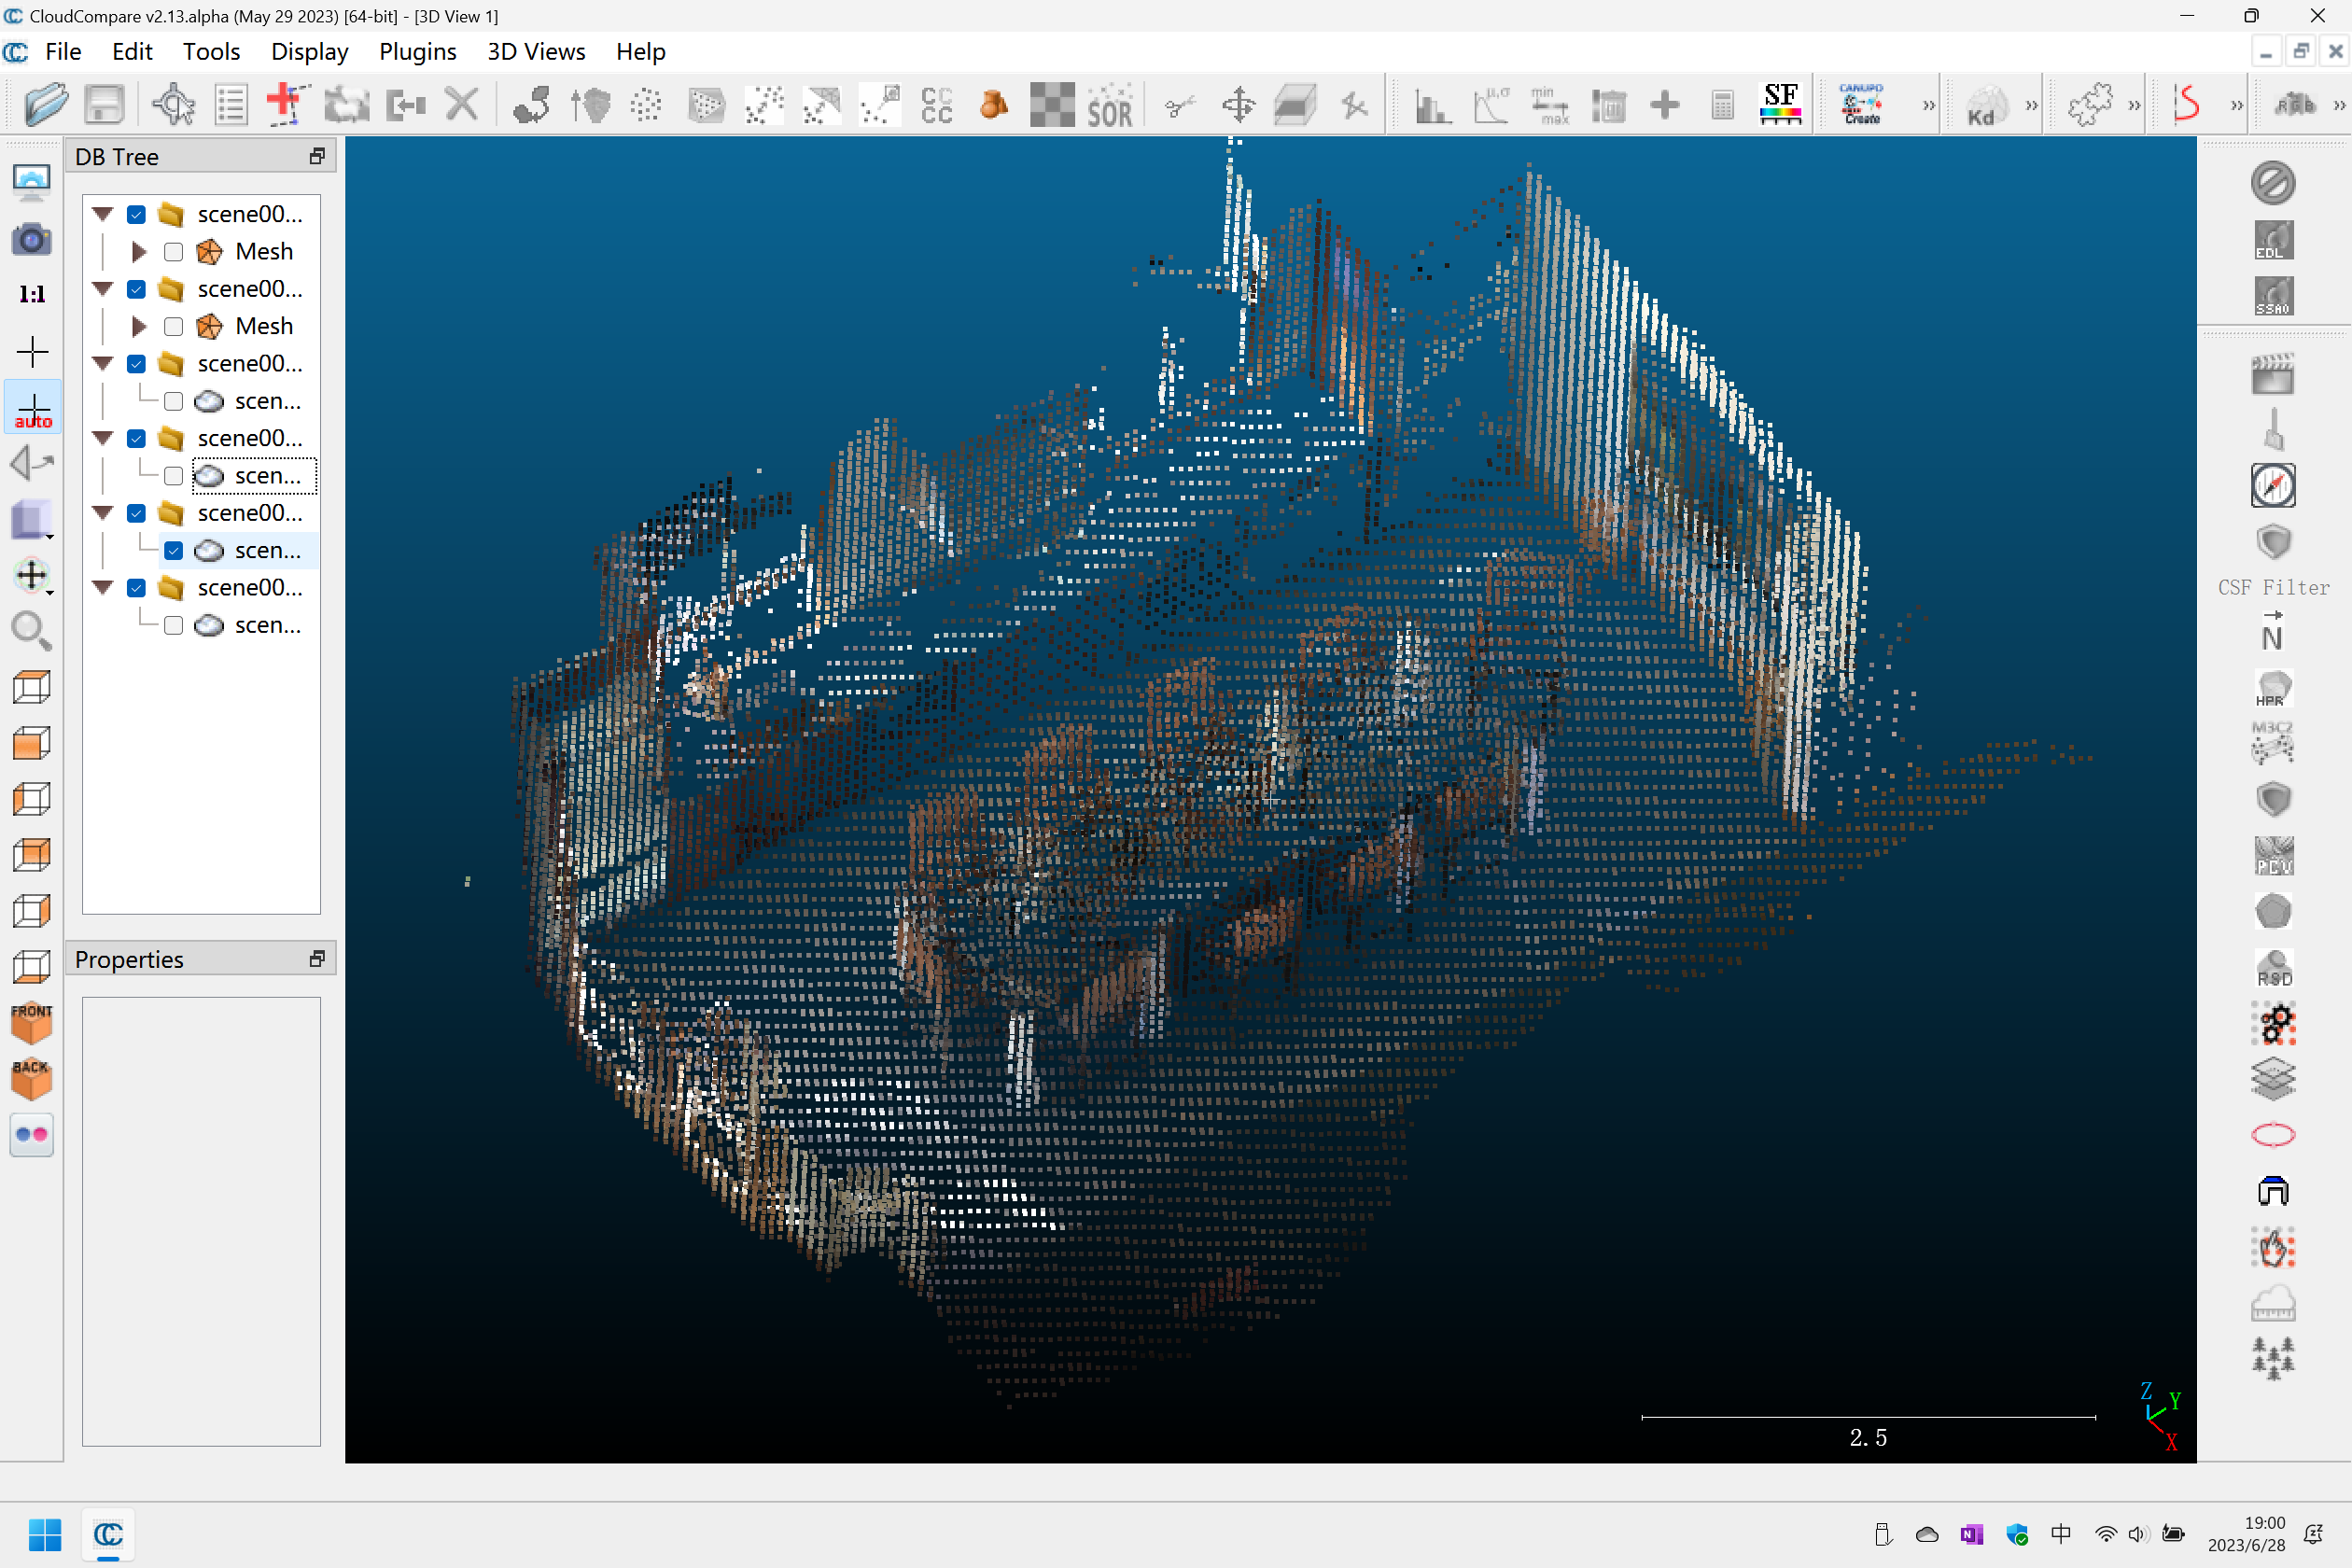
\includegraphics[width=1\textwidth]{figures/result/scene0011_rgb_5cm.png}
		\end{minipage}
	}

	\subfigure[语义信息2cm模型]{
		\begin{minipage}[t]{0.48\linewidth}
			\centering
			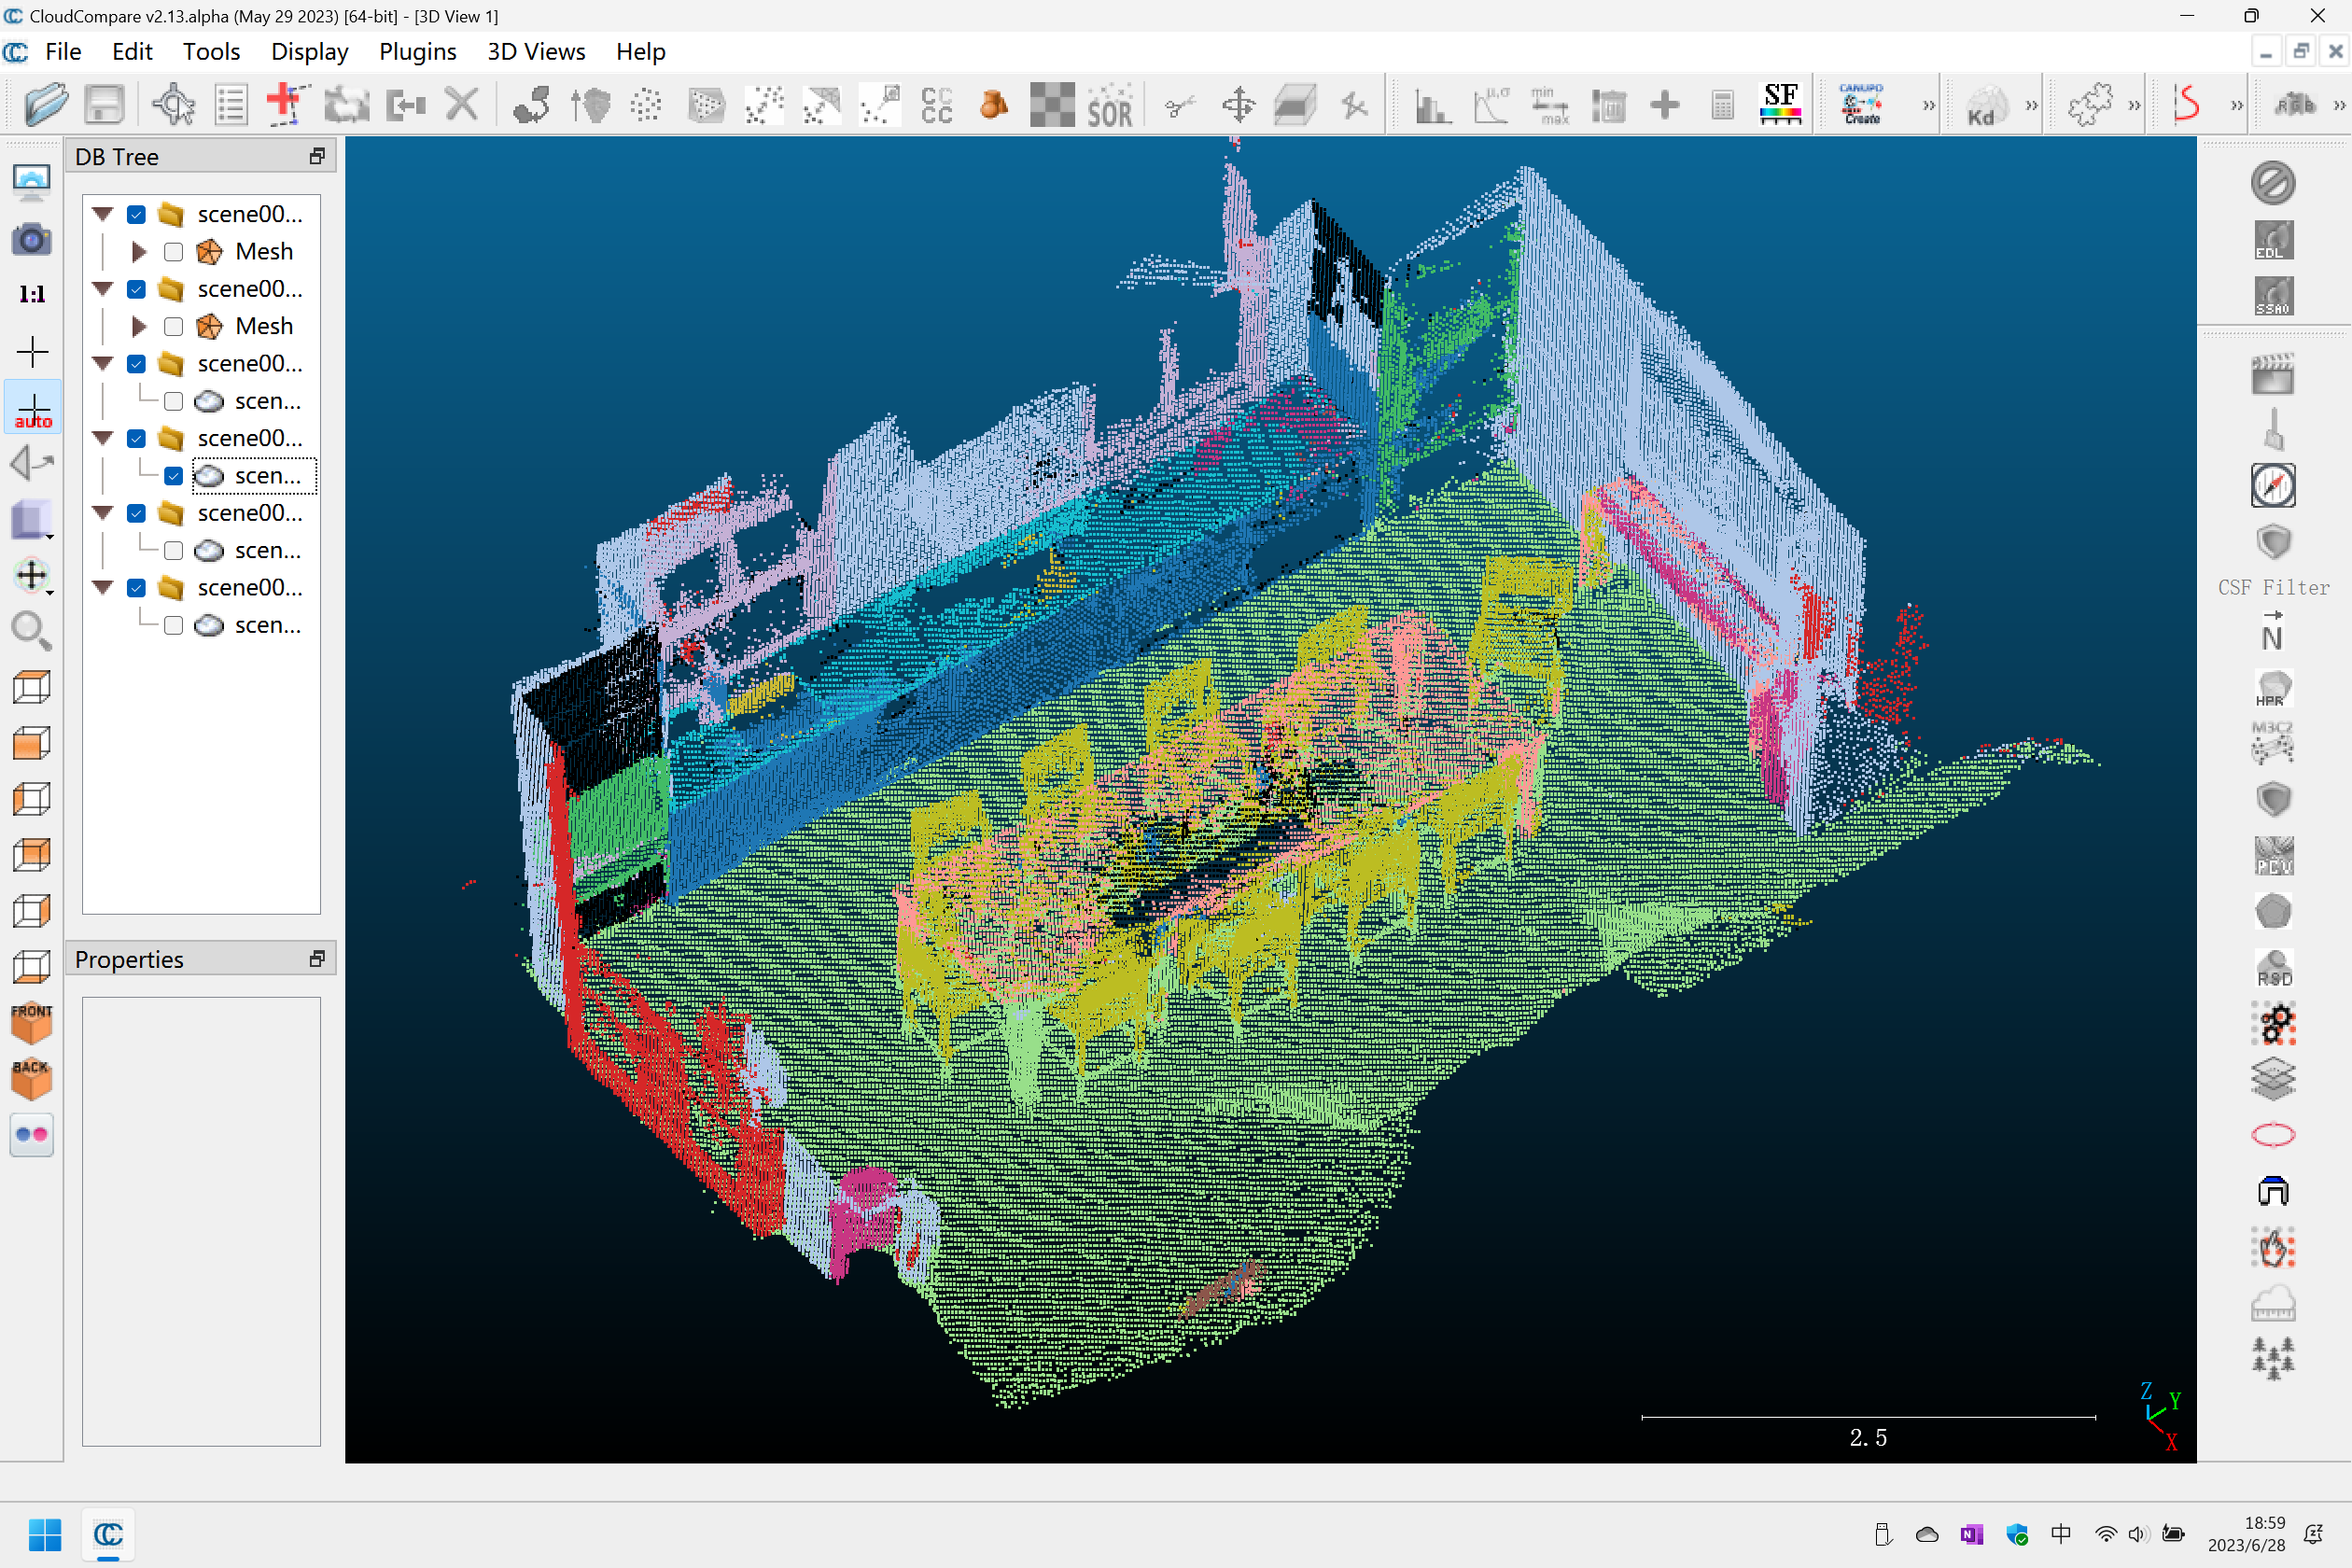
\includegraphics[width=1\textwidth]{figures/result/scene0011_label_2cm.png}
		\end{minipage}
	}
	\subfigure[语义信息5cm模型]{
		\begin{minipage}[t]{0.48\linewidth}
			\centering
			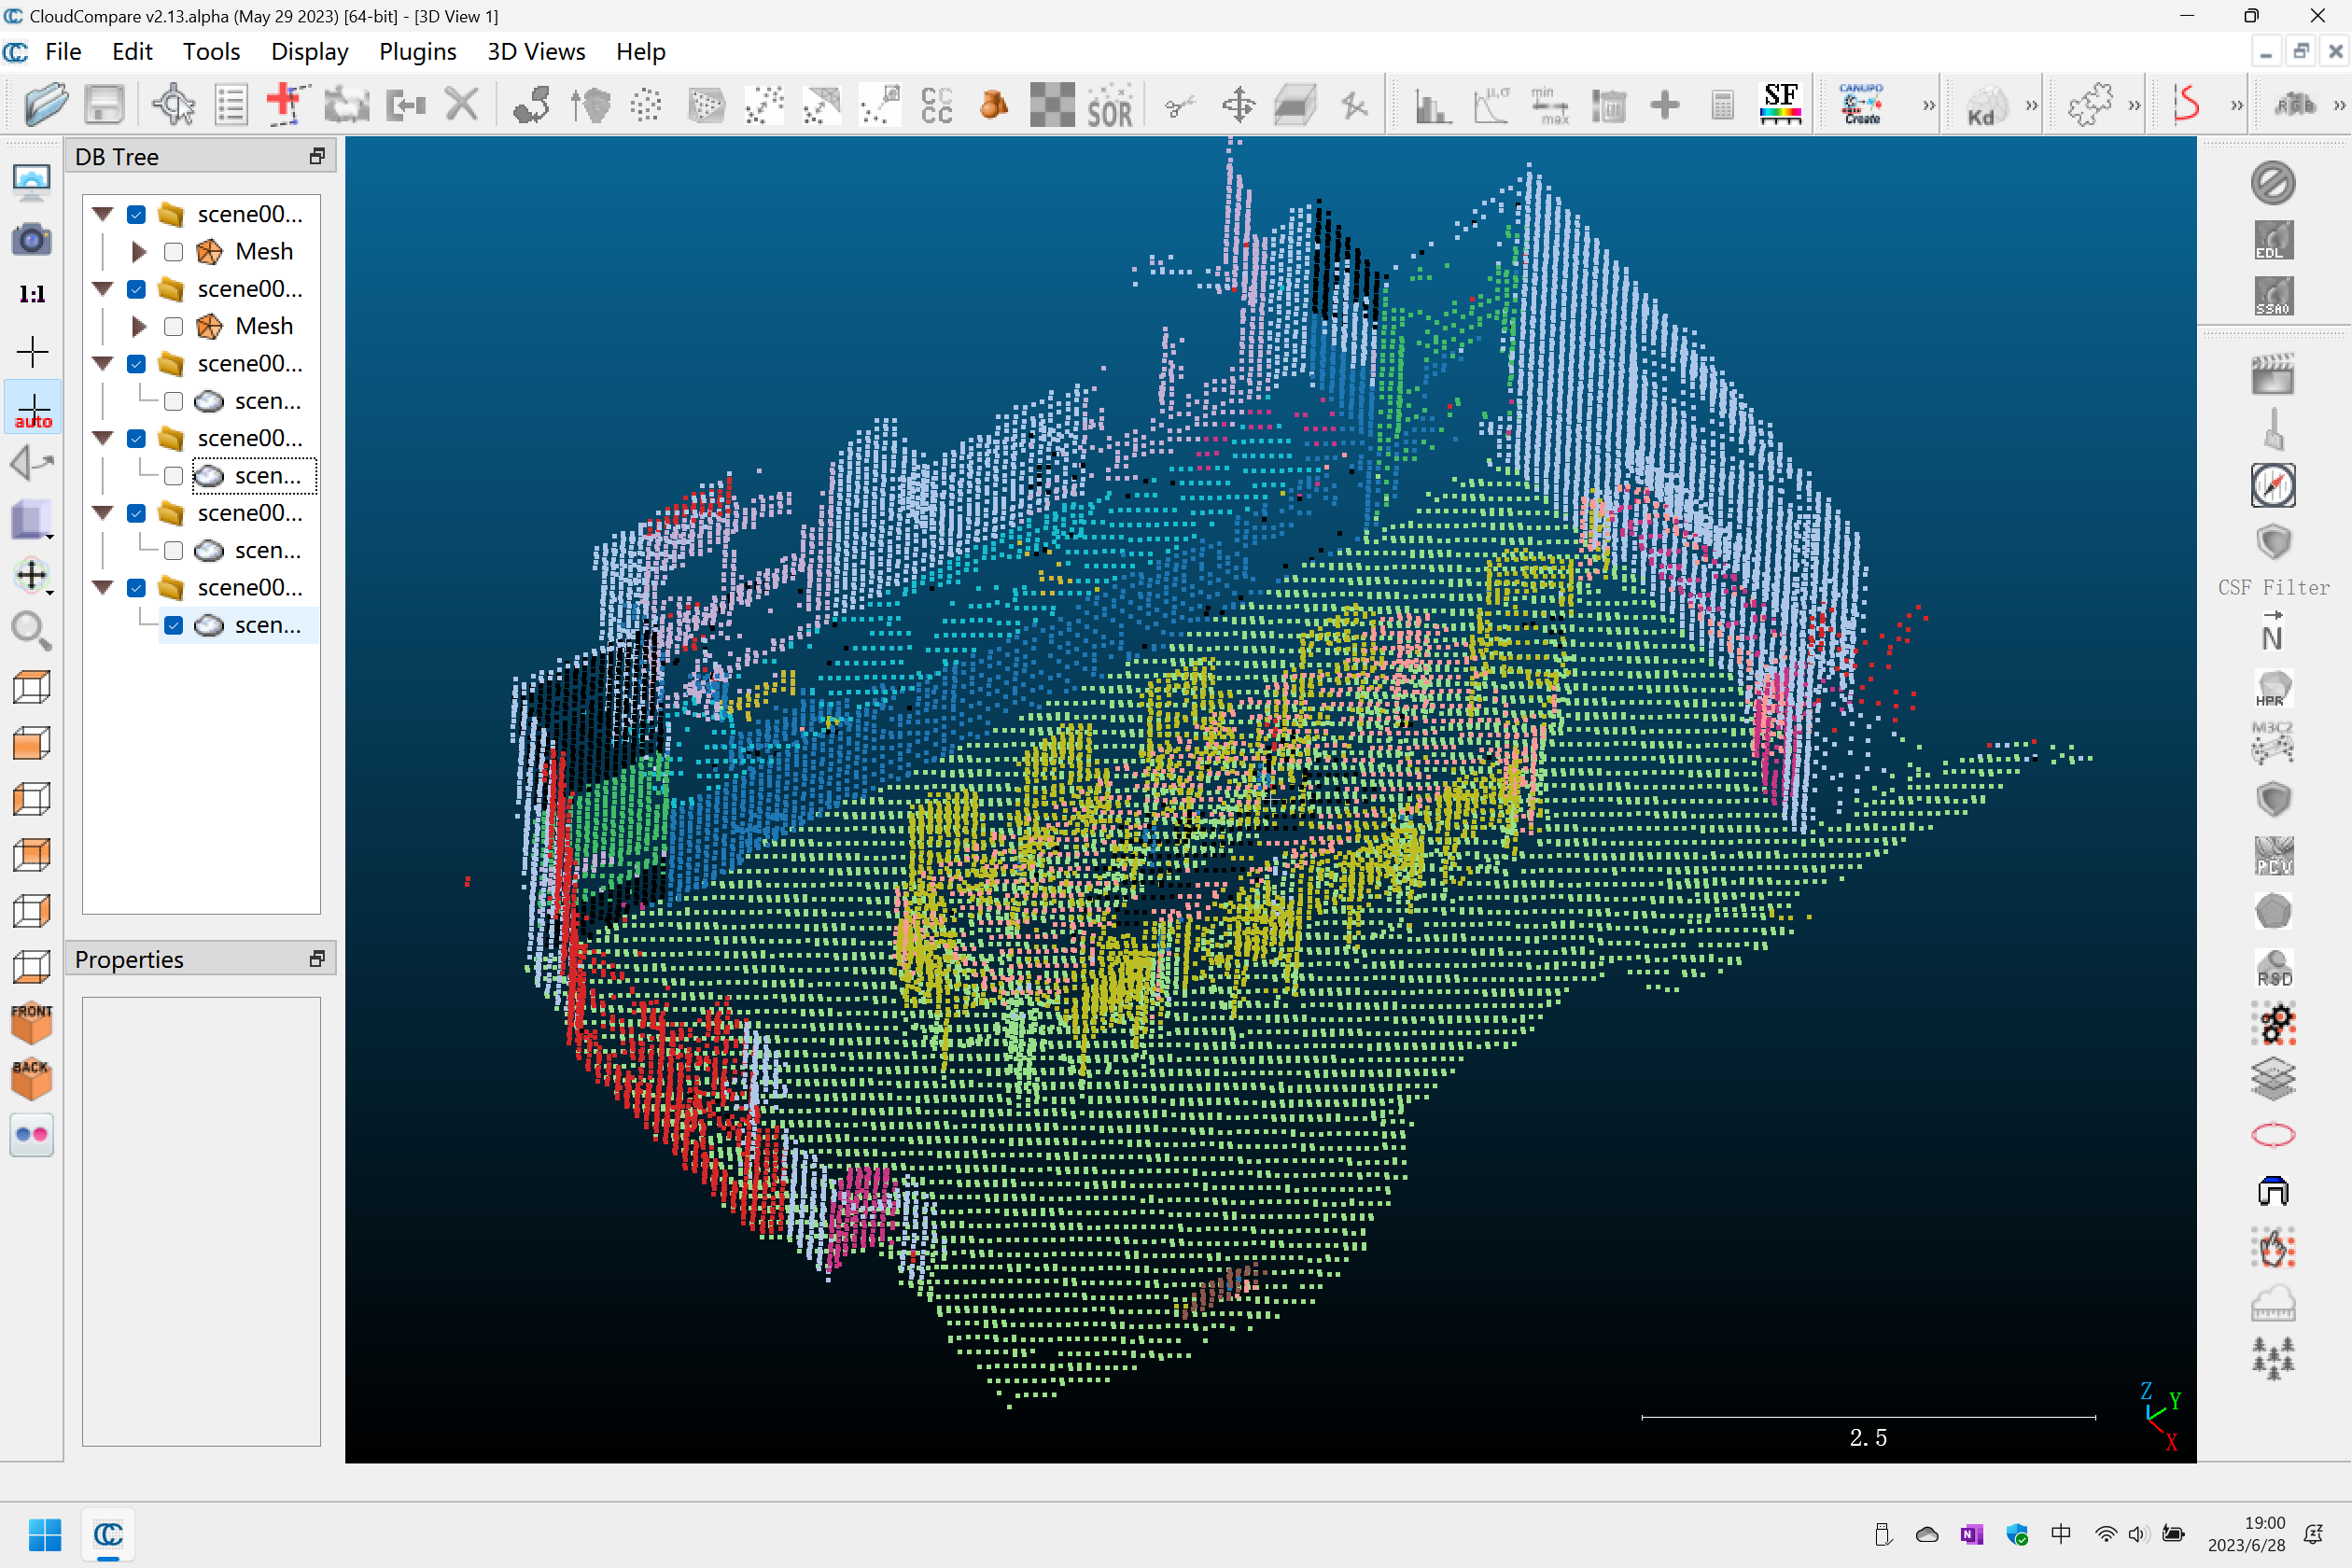
\includegraphics[width=1\textwidth]{figures/result/scene0011_label_5cm.png}
		\end{minipage}
	}
	\caption{模型导出结果}
	\label{fig:export_result}
\end{figure}